\documentclass{article}
\usepackage[utf8]{inputenc}
\usepackage{tikz}

\title{Pagerank Estimation with Deep Graph Networks}
\author{Timo Denk, Samed Güner}
\date{June 2019}

% todo
\usepackage{xargs}                      % Use more than one optional parameter in a new commands
\usepackage[colorinlistoftodos,prependcaption,textsize=tiny]{todonotes}
\newcommandx{\unsure}[2][1=]{\todo[linecolor=red,backgroundcolor=red!25,bordercolor=red,#1]{#2} \PackageWarning{}{#2!}}
\newcommandx{\change}[2][1=]{\todo[linecolor=blue,backgroundcolor=blue!25,bordercolor=blue,#1]{#2}\PackageWarning{}{#2!}}
\newcommandx{\info}[2][1=]{\todo[linecolor=OliveGreen,backgroundcolor=OliveGreen!25,bordercolor=OliveGreen,#1]{#2}\PackageWarning{}{#2!}}
\newcommandx{\improve}[2][1=]{\todo[linecolor=Plum,backgroundcolor=Plum!25,bordercolor=Plum,#1]{#2}\PackageWarning{}{#2!}}
\newcommandx{\thiswillnotshow}[2][1=]{\todo[disable,#1]{#2}\PackageWarning{}{#2!}}

% citing
\usepackage[backend=bibtex,style=alphabetic]{biblatex}
\addbibresource{bibliography.bib}

% new paragraph spacing and indent
\setlength{\parindent}{0pt}
\setlength{\parskip}{6pt}

% line spacing
\renewcommand{\baselinestretch}{1.2}
\usepackage{setspace}

% math
\usepackage{amsmath}
\usepackage{amssymb}  % special set sybmols e.g. for real numbers R
\usepackage{bm}  % bold math
\usepackage{isomath}
\usepackage{amsmath}
\usepackage{subcaption}
\usepackage{amsfonts}
\usepackage{amsthm}
\usepackage{multirow}
\usepackage{colortbl}
\usepackage{booktabs}

% graphics
\usepackage{tikz}
\usepackage{pgfplots}
\usepgfplotslibrary{fillbetween}

% box diagrams
\usepackage{flowchart}
\usetikzlibrary{arrows}

% new paragraph spacing and indent
\setlength{\parindent}{0pt}
\setlength{\parskip}{6pt}

% line spacing
\renewcommand{\baselinestretch}{1.2}
\usepackage{setspace}

% links
\usepackage{url}
\usepackage[colorlinks=true, allcolors=blue]{hyperref}
%\usepackage[htt]{hyphenat}  % enable auto line break for texttt

% plot
\usepackage{pgfplots}

% json listing
\usepackage{listings}

\colorlet{punct}{red!60!black}
\definecolor{background}{HTML}{EEEEEE}
\definecolor{delim}{RGB}{20,105,176}
\colorlet{numb}{magenta!60!black}

\lstdefinelanguage{json}{
	basicstyle=\normalfont\ttfamily,
	numbers=left,
	numberstyle=\scriptsize,
	stepnumber=1,
	numbersep=8pt,
	showstringspaces=false,
	breaklines=true,
	frame=lines,
	backgroundcolor=\color{background},
	literate=
	*{0}{{{\color{numb}0}}}{1}
	{1}{{{\color{numb}1}}}{1}
	{2}{{{\color{numb}2}}}{1}
	{3}{{{\color{numb}3}}}{1}
	{4}{{{\color{numb}4}}}{1}
	{5}{{{\color{numb}5}}}{1}
	{6}{{{\color{numb}6}}}{1}
	{7}{{{\color{numb}7}}}{1}
	{8}{{{\color{numb}8}}}{1}
	{9}{{{\color{numb}9}}}{1}
	{:}{{{\color{punct}{:}}}}{1}
	{,}{{{\color{punct}{,}}}}{1}
	{\{}{{{\color{delim}{\{}}}}{1}
	{\}}{{{\color{delim}{\}}}}}{1}
	{[}{{{\color{delim}{[}}}}{1}
	{]}{{{\color{delim}{]}}}}{1},
}
% credits to Deepl Learning Book
% Spacing between notation sections
\newlength{\notationgap}
\setlength{\notationgap}{1pc}
%%%%% NEW MATH DEFINITIONS %%%%%

% Mark sections of captions for referring to divisions of figures
\newcommand{\figleft}{{\em (Left)}}
\newcommand{\figcenter}{{\em (Center)}}
\newcommand{\figright}{{\em (Right)}}
\newcommand{\figtop}{{\em (Top)}}
\newcommand{\figbottom}{{\em (Bottom)}}
\newcommand{\captiona}{{\em (a)}}
\newcommand{\captionb}{{\em (b)}}
\newcommand{\captionc}{{\em (c)}}
\newcommand{\captiond}{{\em (d)}}

% Highlight a newly defined term
\newcommand{\newterm}[1]{{\bf #1}}


% Figure reference, lower-case.
\def\figref#1{figure~\ref{#1}}
% Figure reference, capital. For start of sentence
\def\Figref#1{Figure~\ref{#1}}
\def\twofigref#1#2{figures \ref{#1} and \ref{#2}}
\def\quadfigref#1#2#3#4{figures \ref{#1}, \ref{#2}, \ref{#3} and \ref{#4}}
% Section reference, lower-case.
\def\secref#1{section~\ref{#1}}
% Section reference, capital.
\def\Secref#1{Section~\ref{#1}}
% Reference to two sections.
\def\twosecrefs#1#2{sections \ref{#1} and \ref{#2}}
% Reference to three sections.
\def\secrefs#1#2#3{sections \ref{#1}, \ref{#2} and \ref{#3}}
% Reference to an equation, lower-case.
\def\eqref#1{equation~\ref{#1}}
% Reference to an equation, upper case
\def\Eqref#1{Equation~\ref{#1}}
% A raw reference to an equation---avoid using if possible
\def\plaineqref#1{\ref{#1}}
% Reference to a chapter, lower-case.
\def\chapref#1{chapter~\ref{#1}}
% Reference to an equation, upper case.
\def\Chapref#1{Chapter~\ref{#1}}
% Reference to a range of chapters
\def\rangechapref#1#2{chapters\ref{#1}--\ref{#2}}
% Reference to an algorithm, lower-case.
\def\algref#1{algorithm~\ref{#1}}
% Reference to an algorithm, upper case.
\def\Algref#1{Algorithm~\ref{#1}}
\def\twoalgref#1#2{algorithms \ref{#1} and \ref{#2}}
\def\Twoalgref#1#2{Algorithms \ref{#1} and \ref{#2}}
% Reference to a part, lower case
\def\partref#1{part~\ref{#1}}
% Reference to a part, upper case
\def\Partref#1{Part~\ref{#1}}
\def\twopartref#1#2{parts \ref{#1} and \ref{#2}}

\def\ceil#1{\lceil #1 \rceil}
\def\floor#1{\lfloor #1 \rfloor}
\def\1{\bm{1}}
\newcommand{\train}{\mathcal{D}}
\newcommand{\valid}{\mathcal{D_{\mathrm{valid}}}}
\newcommand{\test}{\mathcal{D_{\mathrm{test}}}}

\def\eps{{\epsilon}}


% Random variables
\def\reta{{\textnormal{$\eta$}}}
\def\ra{{\textnormal{a}}}
\def\rb{{\textnormal{b}}}
\def\rc{{\textnormal{c}}}
\def\rd{{\textnormal{d}}}
\def\re{{\textnormal{e}}}
\def\rf{{\textnormal{f}}}
\def\rg{{\textnormal{g}}}
\def\rh{{\textnormal{h}}}
\def\ri{{\textnormal{i}}}
\def\rj{{\textnormal{j}}}
\def\rk{{\textnormal{k}}}
\def\rl{{\textnormal{l}}}
% rm is already a command, just don't name any random variables m
\def\rn{{\textnormal{n}}}
\def\ro{{\textnormal{o}}}
\def\rp{{\textnormal{p}}}
\def\rq{{\textnormal{q}}}
\def\rr{{\textnormal{r}}}
\def\rs{{\textnormal{s}}}
\def\rt{{\textnormal{t}}}
\def\ru{{\textnormal{u}}}
\def\rv{{\textnormal{v}}}
\def\rw{{\textnormal{w}}}
\def\rx{{\textnormal{x}}}
\def\ry{{\textnormal{y}}}
\def\rz{{\textnormal{z}}}

% Random vectors
\def\rvepsilon{{\mathbf{\epsilon}}}
\def\rvtheta{{\mathbf{\theta}}}
\def\rva{{\mathbf{a}}}
\def\rvb{{\mathbf{b}}}
\def\rvc{{\mathbf{c}}}
\def\rvd{{\mathbf{d}}}
\def\rve{{\mathbf{e}}}
\def\rvf{{\mathbf{f}}}
\def\rvg{{\mathbf{g}}}
\def\rvh{{\mathbf{h}}}
\def\rvu{{\mathbf{i}}}
\def\rvj{{\mathbf{j}}}
\def\rvk{{\mathbf{k}}}
\def\rvl{{\mathbf{l}}}
\def\rvm{{\mathbf{m}}}
\def\rvn{{\mathbf{n}}}
\def\rvo{{\mathbf{o}}}
\def\rvp{{\mathbf{p}}}
\def\rvq{{\mathbf{q}}}
\def\rvr{{\mathbf{r}}}
\def\rvs{{\mathbf{s}}}
\def\rvt{{\mathbf{t}}}
\def\rvu{{\mathbf{u}}}
\def\rvv{{\mathbf{v}}}
\def\rvw{{\mathbf{w}}}
\def\rvx{{\mathbf{x}}}
\def\rvy{{\mathbf{y}}}
\def\rvz{{\mathbf{z}}}

% Elements of random vectors
\def\erva{{\textnormal{a}}}
\def\ervb{{\textnormal{b}}}
\def\ervc{{\textnormal{c}}}
\def\ervd{{\textnormal{d}}}
\def\erve{{\textnormal{e}}}
\def\ervf{{\textnormal{f}}}
\def\ervg{{\textnormal{g}}}
\def\ervh{{\textnormal{h}}}
\def\ervi{{\textnormal{i}}}
\def\ervj{{\textnormal{j}}}
\def\ervk{{\textnormal{k}}}
\def\ervl{{\textnormal{l}}}
\def\ervm{{\textnormal{m}}}
\def\ervn{{\textnormal{n}}}
\def\ervo{{\textnormal{o}}}
\def\ervp{{\textnormal{p}}}
\def\ervq{{\textnormal{q}}}
\def\ervr{{\textnormal{r}}}
\def\ervs{{\textnormal{s}}}
\def\ervt{{\textnormal{t}}}
\def\ervu{{\textnormal{u}}}
\def\ervv{{\textnormal{v}}}
\def\ervw{{\textnormal{w}}}
\def\ervx{{\textnormal{x}}}
\def\ervy{{\textnormal{y}}}
\def\ervz{{\textnormal{z}}}

% Random matrices
\def\rmA{{\mathbf{A}}}
\def\rmB{{\mathbf{B}}}
\def\rmC{{\mathbf{C}}}
\def\rmD{{\mathbf{D}}}
\def\rmE{{\mathbf{E}}}
\def\rmF{{\mathbf{F}}}
\def\rmG{{\mathbf{G}}}
\def\rmH{{\mathbf{H}}}
\def\rmI{{\mathbf{I}}}
\def\rmJ{{\mathbf{J}}}
\def\rmK{{\mathbf{K}}}
\def\rmL{{\mathbf{L}}}
\def\rmM{{\mathbf{M}}}
\def\rmN{{\mathbf{N}}}
\def\rmO{{\mathbf{O}}}
\def\rmP{{\mathbf{P}}}
\def\rmQ{{\mathbf{Q}}}
\def\rmR{{\mathbf{R}}}
\def\rmS{{\mathbf{S}}}
\def\rmT{{\mathbf{T}}}
\def\rmU{{\mathbf{U}}}
\def\rmV{{\mathbf{V}}}
\def\rmW{{\mathbf{W}}}
\def\rmX{{\mathbf{X}}}
\def\rmY{{\mathbf{Y}}}
\def\rmZ{{\mathbf{Z}}}

% Elements of random matrices
\def\ermA{{\textnormal{A}}}
\def\ermB{{\textnormal{B}}}
\def\ermC{{\textnormal{C}}}
\def\ermD{{\textnormal{D}}}
\def\ermE{{\textnormal{E}}}
\def\ermF{{\textnormal{F}}}
\def\ermG{{\textnormal{G}}}
\def\ermH{{\textnormal{H}}}
\def\ermI{{\textnormal{I}}}
\def\ermJ{{\textnormal{J}}}
\def\ermK{{\textnormal{K}}}
\def\ermL{{\textnormal{L}}}
\def\ermM{{\textnormal{M}}}
\def\ermN{{\textnormal{N}}}
\def\ermO{{\textnormal{O}}}
\def\ermP{{\textnormal{P}}}
\def\ermQ{{\textnormal{Q}}}
\def\ermR{{\textnormal{R}}}
\def\ermS{{\textnormal{S}}}
\def\ermT{{\textnormal{T}}}
\def\ermU{{\textnormal{U}}}
\def\ermV{{\textnormal{V}}}
\def\ermW{{\textnormal{W}}}
\def\ermX{{\textnormal{X}}}
\def\ermY{{\textnormal{Y}}}
\def\ermZ{{\textnormal{Z}}}

% Vectors
\def\vzero{{\bm{0}}}
\def\vone{{\bm{1}}}
\def\vmu{{\bm{\mu}}}
\def\vtheta{{\bm{\theta}}}
\def\va{{\bm{a}}}
\def\vb{{\bm{b}}}
\def\vc{{\bm{c}}}
\def\vd{{\bm{d}}}
\def\ve{{\bm{e}}}
\def\vf{{\bm{f}}}
\def\vg{{\bm{g}}}
\def\vh{{\bm{h}}}
\def\vi{{\bm{i}}}
\def\vj{{\bm{j}}}
\def\vk{{\bm{k}}}
\def\vl{{\bm{l}}}
\def\vm{{\bm{m}}}
\def\vn{{\bm{n}}}
\def\vo{{\bm{o}}}
\def\vp{{\bm{p}}}
\def\vq{{\bm{q}}}
\def\vr{{\bm{r}}}
\def\vs{{\bm{s}}}
\def\vt{{\bm{t}}}
\def\vu{{\bm{u}}}
\def\vv{{\bm{v}}}
\def\vw{{\bm{w}}}
\def\vx{{\bm{x}}}
\def\vy{{\bm{y}}}
\def\vz{{\bm{z}}}

% Elements of vectors
\def\evalpha{{\alpha}}
\def\evbeta{{\beta}}
\def\evepsilon{{\epsilon}}
\def\evlambda{{\lambda}}
\def\evomega{{\omega}}
\def\evmu{{\mu}}
\def\evpsi{{\psi}}
\def\evsigma{{\sigma}}
\def\evtheta{{\theta}}
\def\eva{{a}}
\def\evb{{b}}
\def\evc{{c}}
\def\evd{{d}}
\def\eve{{e}}
\def\evf{{f}}
\def\evg{{g}}
\def\evh{{h}}
\def\evi{{i}}
\def\evj{{j}}
\def\evk{{k}}
\def\evl{{l}}
\def\evm{{m}}
\def\evn{{n}}
\def\evo{{o}}
\def\evp{{p}}
\def\evq{{q}}
\def\evr{{r}}
\def\evs{{s}}
\def\evt{{t}}
\def\evu{{u}}
\def\evv{{v}}
\def\evw{{w}}
\def\evx{{x}}
\def\evy{{y}}
\def\evz{{z}}

% Matrix
\def\mA{{\bm{A}}}
\def\mB{{\bm{B}}}
\def\mC{{\bm{C}}}
\def\mD{{\bm{D}}}
\def\mE{{\bm{E}}}
\def\mF{{\bm{F}}}
\def\mG{{\bm{G}}}
\def\mH{{\bm{H}}}
\def\mI{{\bm{I}}}
\def\mJ{{\bm{J}}}
\def\mK{{\bm{K}}}
\def\mL{{\bm{L}}}
\def\mM{{\bm{M}}}
\def\mN{{\bm{N}}}
\def\mO{{\bm{O}}}
\def\mP{{\bm{P}}}
\def\mQ{{\bm{Q}}}
\def\mR{{\bm{R}}}
\def\mS{{\bm{S}}}
\def\mT{{\bm{T}}}
\def\mU{{\bm{U}}}
\def\mV{{\bm{V}}}
\def\mW{{\bm{W}}}
\def\mX{{\bm{X}}}
\def\mY{{\bm{Y}}}
\def\mZ{{\bm{Z}}}
\def\mBeta{{\bm{\beta}}}
\def\mPhi{{\bm{\Phi}}}
\def\mLambda{{\bm{\Lambda}}}
\def\mSigma{{\bm{\Sigma}}}

% Tensor
\DeclareMathAlphabet{\mathsfit}{\encodingdefault}{\sfdefault}{m}{sl}
\SetMathAlphabet{\mathsfit}{bold}{\encodingdefault}{\sfdefault}{bx}{n}
\newcommand{\tens}[1]{\bm{\mathsfit{#1}}}
\def\tA{{\tens{A}}}
\def\tB{{\tens{B}}}
\def\tC{{\tens{C}}}
\def\tD{{\tens{D}}}
\def\tE{{\tens{E}}}
\def\tF{{\tens{F}}}
\def\tG{{\tens{G}}}
\def\tH{{\tens{H}}}
\def\tI{{\tens{I}}}
\def\tJ{{\tens{J}}}
\def\tK{{\tens{K}}}
\def\tL{{\tens{L}}}
\def\tM{{\tens{M}}}
\def\tN{{\tens{N}}}
\def\tO{{\tens{O}}}
\def\tP{{\tens{P}}}
\def\tQ{{\tens{Q}}}
\def\tR{{\tens{R}}}
\def\tS{{\tens{S}}}
\def\tT{{\tens{T}}}
\def\tU{{\tens{U}}}
\def\tV{{\tens{V}}}
\def\tW{{\tens{W}}}
\def\tX{{\tens{X}}}
\def\tY{{\tens{Y}}}
\def\tZ{{\tens{Z}}}


% Graph
\def\gA{{\mathcal{A}}}
\def\gB{{\mathcal{B}}}
\def\gC{{\mathcal{C}}}
\def\gD{{\mathcal{D}}}
\def\gE{{\mathcal{E}}}
\def\gF{{\mathcal{F}}}
\def\gG{{\mathcal{G}}}
\def\gH{{\mathcal{H}}}
\def\gI{{\mathcal{I}}}
\def\gJ{{\mathcal{J}}}
\def\gK{{\mathcal{K}}}
\def\gL{{\mathcal{L}}}
\def\gM{{\mathcal{M}}}
\def\gN{{\mathcal{N}}}
\def\gO{{\mathcal{O}}}
\def\gP{{\mathcal{P}}}
\def\gQ{{\mathcal{Q}}}
\def\gR{{\mathcal{R}}}
\def\gS{{\mathcal{S}}}
\def\gT{{\mathcal{T}}}
\def\gU{{\mathcal{U}}}
\def\gV{{\mathcal{V}}}
\def\gW{{\mathcal{W}}}
\def\gX{{\mathcal{X}}}
\def\gY{{\mathcal{Y}}}
\def\gZ{{\mathcal{Z}}}

% Sets
\def\sA{{\mathbb{A}}}
\def\sB{{\mathbb{B}}}
\def\sC{{\mathbb{C}}}
\def\sD{{\mathbb{D}}}
% Don't use a set called E, because this would be the same as our symbol
% for expectation.
\def\sF{{\mathbb{F}}}
\def\sG{{\mathbb{G}}}
\def\sH{{\mathbb{H}}}
\def\sI{{\mathbb{I}}}
\def\sJ{{\mathbb{J}}}
\def\sK{{\mathbb{K}}}
\def\sL{{\mathbb{L}}}
\def\sM{{\mathbb{M}}}
\def\sN{{\mathbb{N}}}
\def\sO{{\mathbb{O}}}
\def\sP{{\mathbb{P}}}
\def\sQ{{\mathbb{Q}}}
\def\sR{{\mathbb{R}}}
\def\sS{{\mathbb{S}}}
\def\sT{{\mathbb{T}}}
\def\sU{{\mathbb{U}}}
\def\sV{{\mathbb{V}}}
\def\sW{{\mathbb{W}}}
\def\sX{{\mathbb{X}}}
\def\sY{{\mathbb{Y}}}
\def\sZ{{\mathbb{Z}}}

% Entries of a matrix
\def\emLambda{{\Lambda}}
\def\emA{{A}}
\def\emB{{B}}
\def\emC{{C}}
\def\emD{{D}}
\def\emE{{E}}
\def\emF{{F}}
\def\emG{{G}}
\def\emH{{H}}
\def\emI{{I}}
\def\emJ{{J}}
\def\emK{{K}}
\def\emL{{L}}
\def\emM{{M}}
\def\emN{{N}}
\def\emO{{O}}
\def\emP{{P}}
\def\emQ{{Q}}
\def\emR{{R}}
\def\emS{{S}}
\def\emT{{T}}
\def\emU{{U}}
\def\emV{{V}}
\def\emW{{W}}
\def\emX{{X}}
\def\emY{{Y}}
\def\emZ{{Z}}
\def\emSigma{{\Sigma}}

% entries of a tensor
% Same font as tensor, without \bm wrapper
\newcommand{\etens}[1]{\mathsfit{#1}}
\def\etLambda{{\etens{\Lambda}}}
\def\etA{{\etens{A}}}
\def\etB{{\etens{B}}}
\def\etC{{\etens{C}}}
\def\etD{{\etens{D}}}
\def\etE{{\etens{E}}}
\def\etF{{\etens{F}}}
\def\etG{{\etens{G}}}
\def\etH{{\etens{H}}}
\def\etI{{\etens{I}}}
\def\etJ{{\etens{J}}}
\def\etK{{\etens{K}}}
\def\etL{{\etens{L}}}
\def\etM{{\etens{M}}}
\def\etN{{\etens{N}}}
\def\etO{{\etens{O}}}
\def\etP{{\etens{P}}}
\def\etQ{{\etens{Q}}}
\def\etR{{\etens{R}}}
\def\etS{{\etens{S}}}
\def\etT{{\etens{T}}}
\def\etU{{\etens{U}}}
\def\etV{{\etens{V}}}
\def\etW{{\etens{W}}}
\def\etX{{\etens{X}}}
\def\etY{{\etens{Y}}}
\def\etZ{{\etens{Z}}}

% The true underlying data generating distribution
\newcommand{\pdata}{p_{\rm{data}}}
% The empirical distribution defined by the training set
\newcommand{\ptrain}{\hat{p}_{\rm{data}}}
\newcommand{\Ptrain}{\hat{P}_{\rm{data}}}
% The model distribution
\newcommand{\pmodel}{p_{\rm{model}}}
\newcommand{\Pmodel}{P_{\rm{model}}}
\newcommand{\ptildemodel}{\tilde{p}_{\rm{model}}}
% Stochastic autoencoder distributions
\newcommand{\pencode}{p_{\rm{encoder}}}
\newcommand{\pdecode}{p_{\rm{decoder}}}
\newcommand{\precons}{p_{\rm{reconstruct}}}

\newcommand{\laplace}{\mathrm{Laplace}} % Laplace distribution

\newcommand{\E}{\mathbb{E}}
\newcommand{\Ls}{\mathcal{L}}
\newcommand{\R}{\mathbb{R}}
\newcommand{\emp}{\tilde{p}}
\newcommand{\lr}{\alpha}
\newcommand{\reg}{\lambda}
\newcommand{\rect}{\mathrm{rectifier}}
\newcommand{\softmax}{\mathrm{softmax}}
\newcommand{\sigmoid}{\sigma}
\newcommand{\softplus}{\zeta}
\newcommand{\KL}{D_{\mathrm{KL}}}
\newcommand{\Var}{\mathrm{Var}}
\newcommand{\standarderror}{\mathrm{SE}}
\newcommand{\Cov}{\mathrm{Cov}}
% Wolfram Mathworld says $L^2$ is for function spaces and $\ell^2$ is for vectors
% But then they seem to use $L^2$ for vectors throughout the site, and so does
% wikipedia.
\newcommand{\normlzero}{L^0}
\newcommand{\normlone}{L^1}
\newcommand{\normltwo}{L^2}
\newcommand{\normlp}{L^p}
\newcommand{\normmax}{L^\infty}

\newcommand{\parents}{Pa} % See usage in notation.tex. Chosen to match Daphne's book.

\DeclareMathOperator*{\argmax}{arg\,max}
\DeclareMathOperator*{\argmin}{arg\,min}

\DeclareMathOperator{\sign}{sign}
\DeclareMathOperator{\Tr}{Tr}
\let\ab\allowbreak 


% credits to Deepl Learning Book
% Spacing between notation sections
\newlength{\notationgap}
\setlength{\notationgap}{1pc}
%%%%% NEW MATH DEFINITIONS %%%%%

% Mark sections of captions for referring to divisions of figures
\newcommand{\figleft}{{\em (Left)}}
\newcommand{\figcenter}{{\em (Center)}}
\newcommand{\figright}{{\em (Right)}}
\newcommand{\figtop}{{\em (Top)}}
\newcommand{\figbottom}{{\em (Bottom)}}
\newcommand{\captiona}{{\em (a)}}
\newcommand{\captionb}{{\em (b)}}
\newcommand{\captionc}{{\em (c)}}
\newcommand{\captiond}{{\em (d)}}

% Highlight a newly defined term
\newcommand{\newterm}[1]{{\bf #1}}


% Figure reference, lower-case.
\def\figref#1{figure~\ref{#1}}
% Figure reference, capital. For start of sentence
\def\Figref#1{Figure~\ref{#1}}
\def\twofigref#1#2{figures \ref{#1} and \ref{#2}}
\def\quadfigref#1#2#3#4{figures \ref{#1}, \ref{#2}, \ref{#3} and \ref{#4}}
% Section reference, lower-case.
\def\secref#1{section~\ref{#1}}
% Section reference, capital.
\def\Secref#1{Section~\ref{#1}}
% Reference to two sections.
\def\twosecrefs#1#2{sections \ref{#1} and \ref{#2}}
% Reference to three sections.
\def\secrefs#1#2#3{sections \ref{#1}, \ref{#2} and \ref{#3}}
% Reference to an equation, lower-case.
\def\eqref#1{equation~\ref{#1}}
% Reference to an equation, upper case
\def\Eqref#1{Equation~\ref{#1}}
% A raw reference to an equation---avoid using if possible
\def\plaineqref#1{\ref{#1}}
% Reference to a chapter, lower-case.
\def\chapref#1{chapter~\ref{#1}}
% Reference to an equation, upper case.
\def\Chapref#1{Chapter~\ref{#1}}
% Reference to a range of chapters
\def\rangechapref#1#2{chapters\ref{#1}--\ref{#2}}
% Reference to an algorithm, lower-case.
\def\algref#1{algorithm~\ref{#1}}
% Reference to an algorithm, upper case.
\def\Algref#1{Algorithm~\ref{#1}}
\def\twoalgref#1#2{algorithms \ref{#1} and \ref{#2}}
\def\Twoalgref#1#2{Algorithms \ref{#1} and \ref{#2}}
% Reference to a part, lower case
\def\partref#1{part~\ref{#1}}
% Reference to a part, upper case
\def\Partref#1{Part~\ref{#1}}
\def\twopartref#1#2{parts \ref{#1} and \ref{#2}}

\def\ceil#1{\lceil #1 \rceil}
\def\floor#1{\lfloor #1 \rfloor}
\def\1{\bm{1}}
\newcommand{\train}{\mathcal{D}}
\newcommand{\valid}{\mathcal{D_{\mathrm{valid}}}}
\newcommand{\test}{\mathcal{D_{\mathrm{test}}}}

\def\eps{{\epsilon}}


% Random variables
\def\reta{{\textnormal{$\eta$}}}
\def\ra{{\textnormal{a}}}
\def\rb{{\textnormal{b}}}
\def\rc{{\textnormal{c}}}
\def\rd{{\textnormal{d}}}
\def\re{{\textnormal{e}}}
\def\rf{{\textnormal{f}}}
\def\rg{{\textnormal{g}}}
\def\rh{{\textnormal{h}}}
\def\ri{{\textnormal{i}}}
\def\rj{{\textnormal{j}}}
\def\rk{{\textnormal{k}}}
\def\rl{{\textnormal{l}}}
% rm is already a command, just don't name any random variables m
\def\rn{{\textnormal{n}}}
\def\ro{{\textnormal{o}}}
\def\rp{{\textnormal{p}}}
\def\rq{{\textnormal{q}}}
\def\rr{{\textnormal{r}}}
\def\rs{{\textnormal{s}}}
\def\rt{{\textnormal{t}}}
\def\ru{{\textnormal{u}}}
\def\rv{{\textnormal{v}}}
\def\rw{{\textnormal{w}}}
\def\rx{{\textnormal{x}}}
\def\ry{{\textnormal{y}}}
\def\rz{{\textnormal{z}}}

% Random vectors
\def\rvepsilon{{\mathbf{\epsilon}}}
\def\rvtheta{{\mathbf{\theta}}}
\def\rva{{\mathbf{a}}}
\def\rvb{{\mathbf{b}}}
\def\rvc{{\mathbf{c}}}
\def\rvd{{\mathbf{d}}}
\def\rve{{\mathbf{e}}}
\def\rvf{{\mathbf{f}}}
\def\rvg{{\mathbf{g}}}
\def\rvh{{\mathbf{h}}}
\def\rvu{{\mathbf{i}}}
\def\rvj{{\mathbf{j}}}
\def\rvk{{\mathbf{k}}}
\def\rvl{{\mathbf{l}}}
\def\rvm{{\mathbf{m}}}
\def\rvn{{\mathbf{n}}}
\def\rvo{{\mathbf{o}}}
\def\rvp{{\mathbf{p}}}
\def\rvq{{\mathbf{q}}}
\def\rvr{{\mathbf{r}}}
\def\rvs{{\mathbf{s}}}
\def\rvt{{\mathbf{t}}}
\def\rvu{{\mathbf{u}}}
\def\rvv{{\mathbf{v}}}
\def\rvw{{\mathbf{w}}}
\def\rvx{{\mathbf{x}}}
\def\rvy{{\mathbf{y}}}
\def\rvz{{\mathbf{z}}}

% Elements of random vectors
\def\erva{{\textnormal{a}}}
\def\ervb{{\textnormal{b}}}
\def\ervc{{\textnormal{c}}}
\def\ervd{{\textnormal{d}}}
\def\erve{{\textnormal{e}}}
\def\ervf{{\textnormal{f}}}
\def\ervg{{\textnormal{g}}}
\def\ervh{{\textnormal{h}}}
\def\ervi{{\textnormal{i}}}
\def\ervj{{\textnormal{j}}}
\def\ervk{{\textnormal{k}}}
\def\ervl{{\textnormal{l}}}
\def\ervm{{\textnormal{m}}}
\def\ervn{{\textnormal{n}}}
\def\ervo{{\textnormal{o}}}
\def\ervp{{\textnormal{p}}}
\def\ervq{{\textnormal{q}}}
\def\ervr{{\textnormal{r}}}
\def\ervs{{\textnormal{s}}}
\def\ervt{{\textnormal{t}}}
\def\ervu{{\textnormal{u}}}
\def\ervv{{\textnormal{v}}}
\def\ervw{{\textnormal{w}}}
\def\ervx{{\textnormal{x}}}
\def\ervy{{\textnormal{y}}}
\def\ervz{{\textnormal{z}}}

% Random matrices
\def\rmA{{\mathbf{A}}}
\def\rmB{{\mathbf{B}}}
\def\rmC{{\mathbf{C}}}
\def\rmD{{\mathbf{D}}}
\def\rmE{{\mathbf{E}}}
\def\rmF{{\mathbf{F}}}
\def\rmG{{\mathbf{G}}}
\def\rmH{{\mathbf{H}}}
\def\rmI{{\mathbf{I}}}
\def\rmJ{{\mathbf{J}}}
\def\rmK{{\mathbf{K}}}
\def\rmL{{\mathbf{L}}}
\def\rmM{{\mathbf{M}}}
\def\rmN{{\mathbf{N}}}
\def\rmO{{\mathbf{O}}}
\def\rmP{{\mathbf{P}}}
\def\rmQ{{\mathbf{Q}}}
\def\rmR{{\mathbf{R}}}
\def\rmS{{\mathbf{S}}}
\def\rmT{{\mathbf{T}}}
\def\rmU{{\mathbf{U}}}
\def\rmV{{\mathbf{V}}}
\def\rmW{{\mathbf{W}}}
\def\rmX{{\mathbf{X}}}
\def\rmY{{\mathbf{Y}}}
\def\rmZ{{\mathbf{Z}}}

% Elements of random matrices
\def\ermA{{\textnormal{A}}}
\def\ermB{{\textnormal{B}}}
\def\ermC{{\textnormal{C}}}
\def\ermD{{\textnormal{D}}}
\def\ermE{{\textnormal{E}}}
\def\ermF{{\textnormal{F}}}
\def\ermG{{\textnormal{G}}}
\def\ermH{{\textnormal{H}}}
\def\ermI{{\textnormal{I}}}
\def\ermJ{{\textnormal{J}}}
\def\ermK{{\textnormal{K}}}
\def\ermL{{\textnormal{L}}}
\def\ermM{{\textnormal{M}}}
\def\ermN{{\textnormal{N}}}
\def\ermO{{\textnormal{O}}}
\def\ermP{{\textnormal{P}}}
\def\ermQ{{\textnormal{Q}}}
\def\ermR{{\textnormal{R}}}
\def\ermS{{\textnormal{S}}}
\def\ermT{{\textnormal{T}}}
\def\ermU{{\textnormal{U}}}
\def\ermV{{\textnormal{V}}}
\def\ermW{{\textnormal{W}}}
\def\ermX{{\textnormal{X}}}
\def\ermY{{\textnormal{Y}}}
\def\ermZ{{\textnormal{Z}}}

% Vectors
\def\vzero{{\bm{0}}}
\def\vone{{\bm{1}}}
\def\vmu{{\bm{\mu}}}
\def\vtheta{{\bm{\theta}}}
\def\va{{\bm{a}}}
\def\vb{{\bm{b}}}
\def\vc{{\bm{c}}}
\def\vd{{\bm{d}}}
\def\ve{{\bm{e}}}
\def\vf{{\bm{f}}}
\def\vg{{\bm{g}}}
\def\vh{{\bm{h}}}
\def\vi{{\bm{i}}}
\def\vj{{\bm{j}}}
\def\vk{{\bm{k}}}
\def\vl{{\bm{l}}}
\def\vm{{\bm{m}}}
\def\vn{{\bm{n}}}
\def\vo{{\bm{o}}}
\def\vp{{\bm{p}}}
\def\vq{{\bm{q}}}
\def\vr{{\bm{r}}}
\def\vs{{\bm{s}}}
\def\vt{{\bm{t}}}
\def\vu{{\bm{u}}}
\def\vv{{\bm{v}}}
\def\vw{{\bm{w}}}
\def\vx{{\bm{x}}}
\def\vy{{\bm{y}}}
\def\vz{{\bm{z}}}

% Elements of vectors
\def\evalpha{{\alpha}}
\def\evbeta{{\beta}}
\def\evepsilon{{\epsilon}}
\def\evlambda{{\lambda}}
\def\evomega{{\omega}}
\def\evmu{{\mu}}
\def\evpsi{{\psi}}
\def\evsigma{{\sigma}}
\def\evtheta{{\theta}}
\def\eva{{a}}
\def\evb{{b}}
\def\evc{{c}}
\def\evd{{d}}
\def\eve{{e}}
\def\evf{{f}}
\def\evg{{g}}
\def\evh{{h}}
\def\evi{{i}}
\def\evj{{j}}
\def\evk{{k}}
\def\evl{{l}}
\def\evm{{m}}
\def\evn{{n}}
\def\evo{{o}}
\def\evp{{p}}
\def\evq{{q}}
\def\evr{{r}}
\def\evs{{s}}
\def\evt{{t}}
\def\evu{{u}}
\def\evv{{v}}
\def\evw{{w}}
\def\evx{{x}}
\def\evy{{y}}
\def\evz{{z}}

% Matrix
\def\mA{{\bm{A}}}
\def\mB{{\bm{B}}}
\def\mC{{\bm{C}}}
\def\mD{{\bm{D}}}
\def\mE{{\bm{E}}}
\def\mF{{\bm{F}}}
\def\mG{{\bm{G}}}
\def\mH{{\bm{H}}}
\def\mI{{\bm{I}}}
\def\mJ{{\bm{J}}}
\def\mK{{\bm{K}}}
\def\mL{{\bm{L}}}
\def\mM{{\bm{M}}}
\def\mN{{\bm{N}}}
\def\mO{{\bm{O}}}
\def\mP{{\bm{P}}}
\def\mQ{{\bm{Q}}}
\def\mR{{\bm{R}}}
\def\mS{{\bm{S}}}
\def\mT{{\bm{T}}}
\def\mU{{\bm{U}}}
\def\mV{{\bm{V}}}
\def\mW{{\bm{W}}}
\def\mX{{\bm{X}}}
\def\mY{{\bm{Y}}}
\def\mZ{{\bm{Z}}}
\def\mBeta{{\bm{\beta}}}
\def\mPhi{{\bm{\Phi}}}
\def\mLambda{{\bm{\Lambda}}}
\def\mSigma{{\bm{\Sigma}}}

% Tensor
\DeclareMathAlphabet{\mathsfit}{\encodingdefault}{\sfdefault}{m}{sl}
\SetMathAlphabet{\mathsfit}{bold}{\encodingdefault}{\sfdefault}{bx}{n}
\newcommand{\tens}[1]{\bm{\mathsfit{#1}}}
\def\tA{{\tens{A}}}
\def\tB{{\tens{B}}}
\def\tC{{\tens{C}}}
\def\tD{{\tens{D}}}
\def\tE{{\tens{E}}}
\def\tF{{\tens{F}}}
\def\tG{{\tens{G}}}
\def\tH{{\tens{H}}}
\def\tI{{\tens{I}}}
\def\tJ{{\tens{J}}}
\def\tK{{\tens{K}}}
\def\tL{{\tens{L}}}
\def\tM{{\tens{M}}}
\def\tN{{\tens{N}}}
\def\tO{{\tens{O}}}
\def\tP{{\tens{P}}}
\def\tQ{{\tens{Q}}}
\def\tR{{\tens{R}}}
\def\tS{{\tens{S}}}
\def\tT{{\tens{T}}}
\def\tU{{\tens{U}}}
\def\tV{{\tens{V}}}
\def\tW{{\tens{W}}}
\def\tX{{\tens{X}}}
\def\tY{{\tens{Y}}}
\def\tZ{{\tens{Z}}}


% Graph
\def\gA{{\mathcal{A}}}
\def\gB{{\mathcal{B}}}
\def\gC{{\mathcal{C}}}
\def\gD{{\mathcal{D}}}
\def\gE{{\mathcal{E}}}
\def\gF{{\mathcal{F}}}
\def\gG{{\mathcal{G}}}
\def\gH{{\mathcal{H}}}
\def\gI{{\mathcal{I}}}
\def\gJ{{\mathcal{J}}}
\def\gK{{\mathcal{K}}}
\def\gL{{\mathcal{L}}}
\def\gM{{\mathcal{M}}}
\def\gN{{\mathcal{N}}}
\def\gO{{\mathcal{O}}}
\def\gP{{\mathcal{P}}}
\def\gQ{{\mathcal{Q}}}
\def\gR{{\mathcal{R}}}
\def\gS{{\mathcal{S}}}
\def\gT{{\mathcal{T}}}
\def\gU{{\mathcal{U}}}
\def\gV{{\mathcal{V}}}
\def\gW{{\mathcal{W}}}
\def\gX{{\mathcal{X}}}
\def\gY{{\mathcal{Y}}}
\def\gZ{{\mathcal{Z}}}

% Sets
\def\sA{{\mathbb{A}}}
\def\sB{{\mathbb{B}}}
\def\sC{{\mathbb{C}}}
\def\sD{{\mathbb{D}}}
% Don't use a set called E, because this would be the same as our symbol
% for expectation.
\def\sF{{\mathbb{F}}}
\def\sG{{\mathbb{G}}}
\def\sH{{\mathbb{H}}}
\def\sI{{\mathbb{I}}}
\def\sJ{{\mathbb{J}}}
\def\sK{{\mathbb{K}}}
\def\sL{{\mathbb{L}}}
\def\sM{{\mathbb{M}}}
\def\sN{{\mathbb{N}}}
\def\sO{{\mathbb{O}}}
\def\sP{{\mathbb{P}}}
\def\sQ{{\mathbb{Q}}}
\def\sR{{\mathbb{R}}}
\def\sS{{\mathbb{S}}}
\def\sT{{\mathbb{T}}}
\def\sU{{\mathbb{U}}}
\def\sV{{\mathbb{V}}}
\def\sW{{\mathbb{W}}}
\def\sX{{\mathbb{X}}}
\def\sY{{\mathbb{Y}}}
\def\sZ{{\mathbb{Z}}}

% Entries of a matrix
\def\emLambda{{\Lambda}}
\def\emA{{A}}
\def\emB{{B}}
\def\emC{{C}}
\def\emD{{D}}
\def\emE{{E}}
\def\emF{{F}}
\def\emG{{G}}
\def\emH{{H}}
\def\emI{{I}}
\def\emJ{{J}}
\def\emK{{K}}
\def\emL{{L}}
\def\emM{{M}}
\def\emN{{N}}
\def\emO{{O}}
\def\emP{{P}}
\def\emQ{{Q}}
\def\emR{{R}}
\def\emS{{S}}
\def\emT{{T}}
\def\emU{{U}}
\def\emV{{V}}
\def\emW{{W}}
\def\emX{{X}}
\def\emY{{Y}}
\def\emZ{{Z}}
\def\emSigma{{\Sigma}}

% entries of a tensor
% Same font as tensor, without \bm wrapper
\newcommand{\etens}[1]{\mathsfit{#1}}
\def\etLambda{{\etens{\Lambda}}}
\def\etA{{\etens{A}}}
\def\etB{{\etens{B}}}
\def\etC{{\etens{C}}}
\def\etD{{\etens{D}}}
\def\etE{{\etens{E}}}
\def\etF{{\etens{F}}}
\def\etG{{\etens{G}}}
\def\etH{{\etens{H}}}
\def\etI{{\etens{I}}}
\def\etJ{{\etens{J}}}
\def\etK{{\etens{K}}}
\def\etL{{\etens{L}}}
\def\etM{{\etens{M}}}
\def\etN{{\etens{N}}}
\def\etO{{\etens{O}}}
\def\etP{{\etens{P}}}
\def\etQ{{\etens{Q}}}
\def\etR{{\etens{R}}}
\def\etS{{\etens{S}}}
\def\etT{{\etens{T}}}
\def\etU{{\etens{U}}}
\def\etV{{\etens{V}}}
\def\etW{{\etens{W}}}
\def\etX{{\etens{X}}}
\def\etY{{\etens{Y}}}
\def\etZ{{\etens{Z}}}

% The true underlying data generating distribution
\newcommand{\pdata}{p_{\rm{data}}}
% The empirical distribution defined by the training set
\newcommand{\ptrain}{\hat{p}_{\rm{data}}}
\newcommand{\Ptrain}{\hat{P}_{\rm{data}}}
% The model distribution
\newcommand{\pmodel}{p_{\rm{model}}}
\newcommand{\Pmodel}{P_{\rm{model}}}
\newcommand{\ptildemodel}{\tilde{p}_{\rm{model}}}
% Stochastic autoencoder distributions
\newcommand{\pencode}{p_{\rm{encoder}}}
\newcommand{\pdecode}{p_{\rm{decoder}}}
\newcommand{\precons}{p_{\rm{reconstruct}}}

\newcommand{\laplace}{\mathrm{Laplace}} % Laplace distribution

\newcommand{\E}{\mathbb{E}}
\newcommand{\Ls}{\mathcal{L}}
\newcommand{\R}{\mathbb{R}}
\newcommand{\emp}{\tilde{p}}
\newcommand{\lr}{\alpha}
\newcommand{\reg}{\lambda}
\newcommand{\rect}{\mathrm{rectifier}}
\newcommand{\softmax}{\mathrm{softmax}}
\newcommand{\sigmoid}{\sigma}
\newcommand{\softplus}{\zeta}
\newcommand{\KL}{D_{\mathrm{KL}}}
\newcommand{\Var}{\mathrm{Var}}
\newcommand{\standarderror}{\mathrm{SE}}
\newcommand{\Cov}{\mathrm{Cov}}
% Wolfram Mathworld says $L^2$ is for function spaces and $\ell^2$ is for vectors
% But then they seem to use $L^2$ for vectors throughout the site, and so does
% wikipedia.
\newcommand{\normlzero}{L^0}
\newcommand{\normlone}{L^1}
\newcommand{\normltwo}{L^2}
\newcommand{\normlp}{L^p}
\newcommand{\normmax}{L^\infty}

\newcommand{\parents}{Pa} % See usage in notation.tex. Chosen to match Daphne's book.

\DeclareMathOperator*{\argmax}{arg\,max}
\DeclareMathOperator*{\argmin}{arg\,min}

\DeclareMathOperator{\sign}{sign}
\DeclareMathOperator{\Tr}{Tr}
\let\ab\allowbreak 

\begin{document}

\maketitle

\section{Notation}
\label{notation}
This section introduces the mathematical notations used throughout this document. It is taken from the book \citetitle{Goodfellow-et-al-2016} by \citeauthor{Goodfellow-et-al-2016} (\citeyear{Goodfellow-et-al-2016}).

\vspace{\notationgap}
% Need to use minipage to keep title of table on same page as table
\begin{minipage}{\textwidth}
	% This is a hack to put a little title over the table
	% We cannot use "\section*", etc., they appear in the table of contents.
	% tocdepth does not work on this chapter.
	\centerline{\bf Numbers and Arrays}
	\bgroup
	% The \arraystretch definition here increases the space between rows in the table,
	% so that \displaystyle math has more vertical space.
	\def\arraystretch{1.5}
	\begin{tabular}{cp{3.25in}}
		$\displaystyle a$ & A scalar (integer or real)\\
		$\displaystyle \va$ & A vector\\
		$\displaystyle \mA$ & A matrix\\
		$\displaystyle \tA$ & A tensor\\
		$\displaystyle \mI_n$ & Identity matrix with $n$ rows and $n$ columns\\
		$\displaystyle \mI$ & Identity matrix with dimensionality implied by context\\
		$\displaystyle \ve^{(i)}$ & Standard basis vector $[0,\dots,0,1,0,\dots,0]$ with a 1 at position $i$\\
		$\displaystyle \text{diag}(\va)$ & A square, diagonal matrix with diagonal entries given by $\va$\\
		$\displaystyle \ra$ & A scalar random variable\\
		$\displaystyle \rva$ & A vector-valued random variable\\
		$\displaystyle \rmA$ & A matrix-valued random variable\\
	\end{tabular}
	\egroup
	\index{Scalar}
	\index{Vector}
	\index{Matrix}
	\index{Tensor}
\end{minipage}

\vspace{\notationgap}
\begin{minipage}{\textwidth}
	\centerline{\bf Sets and Graphs}
	\bgroup
	\def\arraystretch{1.5}
	\begin{tabular}{cp{3.25in}}
		$\displaystyle \sA$ & A set\\
		$\displaystyle \R$ & The set of real numbers \\
		% NOTE: do not use \R^+, because it is ambiguous whether:
		% - It includes 0
		% - It includes only real numbers, or also infinity.
		% We usually do not include infinity, so we may explicitly write
		% [0, \infty) to include 0
		% (0, \infty) to not include 0
		$\displaystyle \{0, 1\}$ & The set containing 0 and 1 \\
		$\displaystyle \{0, 1, \dots, n \}$ & The set of all integers between $0$ and $n$\\
		$\displaystyle [a, b]$ & The real interval including $a$ and $b$\\
		$\displaystyle (a, b]$ & The real interval excluding $a$ but including $b$\\
		$\displaystyle \sA \backslash \sB$ & Set subtraction, i.e., the set containing the elements of $\sA$ that are not in $\sB$\\
		$\displaystyle \gG$ & A graph\\
		$\displaystyle \parents_\gG(\ervx_i)$ & The parents of $\ervx_i$ in $\gG$
	\end{tabular}
	\egroup
	\index{Scalar}
	\index{Vector}
	\index{Matrix}
	\index{Tensor}
	\index{Graph}
	\index{Set}
\end{minipage}

\vspace{\notationgap}
\begin{minipage}{\textwidth}
	\centerline{\bf Indexing}
	\bgroup
	\def\arraystretch{1.5}
	\begin{tabular}{cp{3.25in}}
		$\displaystyle \eva_i$ & Element $i$ of vector $\va$, with indexing starting at 1 \\
		$\displaystyle \eva_{-i}$ & All elements of vector $\va$ except for element $i$ \\
		$\displaystyle \emA_{i,j}$ & Element $i, j$ of matrix $\mA$ \\
		$\displaystyle \mA_{i, :}$ & Row $i$ of matrix $\mA$ \\
		$\displaystyle \mA_{:, i}$ & Column $i$ of matrix $\mA$ \\
		$\displaystyle \etA_{i, j, k}$ & Element $(i, j, k)$ of a 3-D tensor $\tA$\\
		$\displaystyle \tA_{:, :, i}$ & 2-D slice of a 3-D tensor\\
		$\displaystyle \erva_i$ & Element $i$ of the random vector $\rva$ \\
	\end{tabular}
	\egroup
\end{minipage}

\vspace{\notationgap}
\begin{minipage}{\textwidth}
	\centerline{\bf Linear Algebra Operations}
	\bgroup
	\def\arraystretch{1.5}
	\begin{tabular}{cp{3.25in}}
		$\displaystyle \mA^\top$ & Transpose of matrix $\mA$ \\
		$\displaystyle \mA^+$ & Moore-Penrose pseudoinverse of $\mA$\\
		$\displaystyle \mA \odot \mB $ & Element-wise (Hadamard) product of $\mA$ and $\mB$ \\
		% Wikipedia uses \circ for element-wise multiplication but this could be confused with function composition
		$\displaystyle \mathrm{det}(\mA)$ & Determinant of $\mA$ \\
	\end{tabular}
	\egroup
	\index{Transpose}
	\index{Element-wise product|see {Hadamard product}}
	\index{Hadamard product}
	\index{Determinant}
\end{minipage}

\vspace{\notationgap}
\begin{minipage}{\textwidth}
	\centerline{\bf Calculus}
	\bgroup
	\def\arraystretch{1.5}
	\begin{tabular}{cp{3.25in}}
		% NOTE: the [2ex] on the next line adds extra height to that row of the table.
		% Without that command, the fraction on the first line is too tall and collides
		% with the fraction on the second line.
		$\displaystyle\frac{d y} {d x}$ & Derivative of $y$ with respect to $x$\\ [2ex]
		$\displaystyle \frac{\partial y} {\partial x} $ & Partial derivative of $y$ with respect to $x$ \\
		$\displaystyle \nabla_\vx y $ & Gradient of $y$ with respect to $\vx$ \\
		$\displaystyle \nabla_\mX y $ & Matrix derivatives of $y$ with respect to $\mX$ \\
		$\displaystyle \nabla_\tX y $ & Tensor containing derivatives of $y$ with respect to $\tX$ \\
		$\displaystyle \frac{\partial f}{\partial \vx} $ & Jacobian matrix $\mJ \in \R^{m\times n}$ of $f: \R^n \rightarrow \R^m$\\
		$\displaystyle \nabla_\vx^2 f(\vx)\text{ or }\mH( f)(\vx)$ & The Hessian matrix of $f$ at input point $\vx$\\
		$\displaystyle \int f(\vx) d\vx $ & Definite integral over the entire domain of $\vx$ \\
		$\displaystyle \int_\sS f(\vx) d\vx$ & Definite integral with respect to $\vx$ over the set $\sS$ \\
	\end{tabular}
	\egroup
	\index{Derivative}
	\index{Integral}
	\index{Jacobian matrix}
	\index{Hessian matrix}
\end{minipage}

\vspace{\notationgap}
\begin{minipage}{\textwidth}
	\centerline{\bf Probability and Information Theory}
	\bgroup
	\def\arraystretch{1.5}
	\begin{tabular}{cp{3.25in}}
		$\displaystyle \ra \bot \rb$ & The random variables $\ra$ and $\rb$ are independent\\
		$\displaystyle \ra \bot \rb \mid \rc $ & They are conditionally independent given $\rc$\\
		$\displaystyle P(\ra)$ & A probability distribution over a discrete variable\\
		$\displaystyle p(\ra)$ & A probability distribution over a continuous variable, or over
		a variable whose type has not been specified\\
		$\displaystyle \ra \sim P$ & Random variable $\ra$ has distribution $P$\\% so thing on left of \sim should always be a random variable, with name beginning with \r
		$\displaystyle  \E_{\rx\sim P} [ f(x) ]\text{ or } \E f(x)$ & Expectation of $f(x)$ with respect to $P(\rx)$ \\
		$\displaystyle \Var(f(x)) $ &  Variance of $f(x)$ under $P(\rx)$ \\
		$\displaystyle \Cov(f(x),g(x)) $ & Covariance of $f(x)$ and $g(x)$ under $P(\rx)$\\
		$\displaystyle H(\rx) $ & Shannon entropy of the random variable $\rx$\\
		$\displaystyle \KL ( P \Vert Q ) $ & Kullback-Leibler divergence of P and Q \\
		$\displaystyle \mathcal{N} ( \vx ; \vmu , \mSigma)$ & Gaussian distribution %
		over $\vx$ with mean $\vmu$ and covariance $\mSigma$ \\
	\end{tabular}
	\egroup
	\index{Independence}
	\index{Conditional independence}
	\index{Variance}
	\index{Covariance}
	\index{Kullback-Leibler divergence}
	\index{Shannon entropy}
\end{minipage}

\vspace{\notationgap}
\begin{minipage}{\textwidth}
	\centerline{\bf Functions}
	\bgroup
	\def\arraystretch{1.5}
	\begin{tabular}{cp{3.25in}}
		$\displaystyle f: \sA \rightarrow \sB$ & The function $f$ with domain $\sA$ and range $\sB$\\
		$\displaystyle f \circ g $ & Composition of the functions $f$ and $g$ \\
		$\displaystyle f(\vx ; \vtheta) $ & A function of $\vx$ parametrized by $\vtheta$.
		(Sometimes we write $f(\vx)$ and omit the argument $\vtheta$ to lighten notation) \\
		$\displaystyle \log x$ & Natural logarithm of $x$ \\
		$\displaystyle \sigma(x)$ & Logistic sigmoid, $\displaystyle \frac{1} {1 + \exp(-x)}$ \\
		$\displaystyle \zeta(x)$ & Softplus, $\log(1 + \exp(x))$ \\
		$\displaystyle || \vx ||_p $ & $\normlp$ norm of $\vx$ \\
		$\displaystyle || \vx || $ & $\normltwo$ norm of $\vx$ \\
		$\displaystyle x^+$ & Positive part of $x$, i.e., $\max(0,x)$\\
		$\displaystyle \1_\mathrm{condition}$ & is 1 if the condition is true, 0 otherwise\\
	\end{tabular}
	\egroup
	\index{Sigmoid}
	\index{Softplus}
	\index{Norm}
\end{minipage}

Sometimes we use a function $f$ whose argument is a scalar but apply
it to a vector, matrix, or tensor: $f(\vx)$, $f(\mX)$, or $f(\tX)$.
This denotes the application of $f$ to the
array element-wise. For example, if $\tC = \sigma(\tX)$, then $\etC_{i,j,k} = \sigma(\etX_{i,j,k})$
for all valid values of $i$, $j$ and $k$.


\vspace{\notationgap}
\begin{minipage}{\textwidth}
	\centerline{\bf Datasets and Distributions}
	\bgroup
	\def\arraystretch{1.5}
	\begin{tabular}{cp{3.25in}}
		$\displaystyle \pdata$ & The data generating distribution\\
		$\displaystyle \ptrain$ & The empirical distribution defined by the training set\\
		$\displaystyle \sX$ & A set of training examples\\
		$\displaystyle \vx^{(i)}$ & The $i$-th example (input) from a dataset\\
		$\displaystyle y^{(i)}\text{ or }\vy^{(i)}$ & The target associated with $\vx^{(i)}$ for supervised learning\\
		$\displaystyle \mX$ & The $m \times n$ matrix with input example $\vx^{(i)}$ in row $\mX_{i,:}$\\
	\end{tabular}
	\egroup
\end{minipage}
\section{Introduction}
\label{section:introduction}

The world wide web has evolved to become a common source of information and entertainment for people from all around the globe. The number of active websites exceeds 100 million by far. People commonly access these websites through the internet using a webbrowser on their computer or hand-held devices and consume the content in graphical or auditory format.

Some website attrackt more visitors than others. As of January 2018, the Alexa page ranking\footnote{The top 500 sites on the web: \url{https://www.alexa.com/topsites}} lists \url{google.com}, \url{youtube.com}, \url{facebook.com}, \url{baidu.com}, and \url{wikipedia.org} as the top five websites. Ordering websites by their popularity can be done in different ways: One might think of the total number of links pointing to a website, the visitor count, visitor count combined with the average time people spend, and other measures.

Newly published websites will initially be assigned a low rank, until their popularity grows and the statistic reflects that. An experienced user, however, might be able to have a rough feeling for whether a website they see has potential to become popular or not, solely based on its content and look. To the best of our knowledge, there is a shortcoming in tools, which estimate the expected popularity of a website, thereby replicating the behavioral patterns of a human observer.

In this work we model a pagerank estimator using methods of computer vision. More specifically, we train a graph network with convolutional building blocks to \textit{look} at screenshots of web pages of a domain and output the expected popularity.

The world wide web has been designed with hyperlinks. They allow users to navigate between web pages. A website typically consists of several web pages, which (often, but not necessarily) point to each other with hyperlinks. Such a website can be interpreted as a graph, where nodes correspond to web pages and edges to hyperlinks connecting two of them. We try to exploit the information contained in the graph structure by applying graph networks to the ranking problem.

Traversing the web page graph of the internet or a single website is referred to as crawling. In order to create a screenshot dataset that contains the meta information we want, we have developed a webcrawler. It is documented in this article.

Our main contributions are:
\begin{itemize}
\item Creation and release of a pagerank dataset with two versions: (v1) A single screenshot for each of the top 100k websites and (v2) 100k graphs, where each graph represents one of the websites with screenshots and meta data.
\item Application of graph networks to the problem of pagerank prediction.
\end{itemize}

This work is a student research project of two students of Applied Computer Science, carried out at Coorporative State University Baden-Wuerttemberg, Karlsruhe.

The remainder of this document is structured as follows: \todo{Write one sentence per section.}

The mathematical notation used throughout this document follows the one defined in the chapter \textit{Notation} of the Deep Learning book by \cite{goodfellow:dlbook}.


\section{Background}
\label{sec:background}

\subsection{Learning to Rank}
\label{sec:learningtorank}

\textit{Learning to rank} is the application of machine learning to the creation of models that can rank. Ranking, in its most general form, is the ordering of a collection of documents (also referred to as samples). The book \textit{Learning to Rank for Information Retrieval} by \cite{liu2009learningtorank} enumerates three distinguishable approaches to phrasing and solving ranking problems. They are referred to as pointwise, pairwise, and listwise, and shall be explained briefly in the following. The second part of this section deals with ranking metrics which are used to evaluate the performance of ranking model, i.e. the quality of its ranking.

The \textbf{pointwise approach} deals with models that determine the rank of a single sample. It can be subdivided into the three subcategories (1) regression based, (2) classification based, and (3) ordinal regression based. For (1), the problem is considered a regression problem, where the rank of a sample is interpreted as a point on the real number line which the model seeks to predict correctly. With (2), the ranks are discrete and considered classes, for a given input, the model predicts a class which can be mapped to a rank. Ranks can also be grouped into bins, such that an entire range of adjacent ranks corresponds to a single class. While the classes in (2) do not have an ordering that is necessarily apparent to the model, the third subcategory (3) takes the ordinal relationship of ranks into account. The goal is to find a scoring functions such that thresholds can be found to distinguish the outputs into the different, ordered categories.

A possible loss function for pointwise training is to interpret the scaled and rounded model output $y\in\mathbb{R}$ as the predicted rank of an input. A loss function could simply penalize divergence from the target output $\hat{y}\in\mathbb{R}$, e.g. in a quadratic fashion, $(y-\hat{y})^2$.

Opposed to the pointwise approach, the \textbf{pairwise approach} does not seek to predict the rank of a single sample. Instead the focus is on predicting the relative order between two given samples, i.e. whether the first sample $\bm{x}^{(i)}$ has a greater or a lower rank than the second one $\bm{x}^{(j)}$. This problem can be considered a binary classification task on a tuple input $(\bm{x}^{(i)},\bm{x}^{(j)})$, where the first class means $\bm{x}^{(i)}\triangleright \bm{x}^{(j)}$ ($\bm{x}^{(i)}$ has a higher rank than $\bm{x}^{(j)}$) and the second class means $\bm{x}^{(i)}\triangleleft \bm{x}^{(j)}$.

\cite{Burges:learningtorankwithsgd} propose a probabilistic cost function for pairwise training. 
They represent the ground truth as a matrix $\bm{\overline{P}}\in[0,1]^{m\times m}$, where $\overline{P}_{i,j}$ is the probability of sample $\bm{x}^{(i)}$ to have a higher rank than $\bm{x}^{(j)}$, i.e. $P(\bm{x}^{(i)}\triangleright \bm{x}^{(j)})$. 
The model itself is a function $f:\mathbb{R}^d\rightarrow\mathbb{R}$ mapping a sample $\bm{x}^{(i)}$ to a scalar. The loss for two given samples $\bm{x}^{(i)}$ and $\bm{x}^{(j)}$ is defined as
\begin{align}
-\overline{P}_{i,j}\left(f\left(\bm{x}^{(i)}\right)-f\left(\bm{x}^{(j)}\right)\right)+\log\left(1+e^{f\left(\bm{x}^{(i)}\right)-f\left(\bm{x}^{(j)}\right)}\right)
\end{align}
This formulation has some favorable properties: It allows for uncertainty in the relative ordering of items in that the $\bm{\overline{P}}$ is a probability and could be e.g. $\overline{P}_{i,j}=\frac{1}{2}$, if the relative ranking of two items was unknown. Furthermore, the loss asymptotes to a linear function. According to the authors, this is likely to be more robust with noisy labels than a quadratic cost.

The \textbf{listwise approach} deals with models taking an entire list of samples as their input, with the goal of ordering them. This can be either done by mapping them to real values and penalizing wrong ordering, or mapping the samples discretely to a permutation.

In real world applications, the training of ranking models can be much more complicated. For example, updating a ranking model based on what users click leads to wrong updates because the feedback from users is biased. \cite{unbiasedlearningtorank} deal with that problem and propose \textit{unbiased learning to rank}. This is, however, beyond the scope of this work, because we do not deal with direct user feedback.

Once a model has produced a ranking, it must be evaluated. Since the magnitude of a loss function is ofter rather less meaningful, other measures, so called \textbf{ranking metrics}, have been defined. \cite{tfranking} name four, namely \textit{Mean Reciprocal Rank (MRR)}, average of positions of examples weighted by their relevance values (\textit{ARP}), \textit{Discounted Cumulative Gain (DCG)}, and \textit{Normalized DCG (NDCG)}. They also make the important point that ``in ranking, it is preferable to have fewer errors at higher ranked positions than at the lower ranked positions, which is reflected in many metrics''.

\subsection{Graph Networks}
\label{sec:graphnetworks}

The most basic type of neural network, consisting solely of fully connected layers, converts a vector of fixed size into another vector of fixed size.
In contrast, convolutional neural networks (CNNs) can convert variably-sized inputs into variably-sized outputs. In image classification or segmentation tasks, the inputs are often scaled to a fixed size and the convolutional layers serve as feature extractors for a fully-connected classification head.
Recurrent neural networks can convert a sequence of vectors into another sequence.

While some of those neural network types \textit{can} handle variably-sized inputs, they do not deal with sets very well: Consider for instance an (unordered) set of images and the task to assign a single label to the entire set. All architectures from above could be applied to that task by simply concatenating all the images into one large vector. However, they would implicitly try to assign a semantic meaning to the ordering in which the samples are being presented to them (relational inductive bias). One could augment the dataset by shuffling the samples of a set before concatenating them but that does not solve the underlying problem. Alternatively, one might process the images in the set individually and combine the outputs. This setup has the drawback that information exchange between internal representations of the model cannot take place. The feature representation of one image cannot influence the processing of other images, which could, however, be a requirement when dealing with a set of images.

Graph networks are designed to handle graphs and sets naturally. They can deal with any size of graph and do not regard the ordering of nodes. While processing the nodes, information can freely flow between them. \cite{deepmind:graphnets} have brought several different types of graph networks under a common hood. We follow their notation and will recapitulate the relevant parts in the following paragraphs. That is the formal definition of a directed, attributed multi-graph with a global attribute, as well as the definition of graph networks.

Let a graph $G$ be a 3-tuple $G=\left(\bm{u},\mathbb{V},\mathbb{E}\right)$, where $\bm{u}$ is a vector of global attributes.
$\mathbb{V}=\left\{\bm{v}_i\right\}_{i=1}^{N^{(v)}}$ is a set of $N^{(v)}$ nodes (also referred to as vertices), each consisting solely of an attribute vector.
$\mathbb{E}=\left\{\left(\bm{e}_k,r_k,s_k\right)\right\}_{k=1}^{N^{(e)}}$ is a set of $N^{(e)}$ edges, each of which connects a sender node $\bm{v}_{s_k}$ to a receiver node $\bm{v}_{r_k}$, and contains an attribute vector $\bm{e}_k$.

The attribute vectors $\bm{u}$, $\bm{v}_i$, and $\bm{e}_k$ can contain any kind of information. In fact they could even be graphs themselves.

Graph networks (GN) are neural networks that contain at least one GN block. \cite{deepmind:graphnets} describe it as follows: A GN block contains three update functions, $\phi$, and three aggregation functions, $\rho$,
\begin{align}
    \bm{e}'_k=&\phi^e\left(\bm{e}_k,\bm{v}_{r_k},\bm{v}_{s_k},\bm{u}\right)\\
    \bm{\overline{e}}'_i=&\rho^{e\rightarrow v}\left(\mathbb{E}'_i\right)\\
    \bm{v}'_i=&\phi^v\left(\bm{\overline{e}}'_i,\bm{v}_i,\bm{u}\right)\\
    \bm{\overline{e}}'=&\rho^{e\rightarrow u}\left(\mathbb{E}'\right)\\
    \bm{\overline{v}}'=&\rho^{v\rightarrow u}\left(\mathbb{V}'\right)\\
    \bm{u}'=&\phi^u\left(\bm{\overline{e}}',\bm{\overline{v}},\bm{u}\right)\,,
\end{align}
where $\mathbb{E}'_i=\left\{\left(\bm{e}'_k,r_k,s_k\right)\right\}_{r_k=i,k=1}^{N^{(e)}}$ is the set of all edges pointing to the $i$th node; $\mathbb{V}'=\left\{\bm{v}'_i\right\}_{i=1}^{N^{(v)}}$; $\mathbb{E}'=\bigcup_i\mathbb{E}'_i$.

\begin{enumerate}
    \item $\phi^e$ is the \textbf{edge update function} and applied to every edge in the graph. For the $k$th edge it computes a new attribute vector $\bm{e}'_k$ based on the previous state $\bm{e}_k$, the attributes of the two nodes that this edge connects, namely $\bm{v}_{r_k}$ and $\bm{v}_{s_k}$, and the global state $\bm{u}$.
    \item $\rho^{e\rightarrow v}$ is the \textbf{edge aggregation function} and applied once for every node in the graph. It computes an aggregation of all edges pointing to the $i$th node.
    \item $\phi^v$ is the \textbf{node update function}. It is applied to every node in the graph and computes the new attribute vector $\bm{v}'_i$ based on the aggregation of all edges pointing to the node, the previous state of the node, and the global state.
    \item $\rho^{e\rightarrow u}$ is the \textbf{global edge aggregation function} which computes an aggregation $\bm{\overline{e}}'$ of all edges in the graph.
    \item $\rho^{v\rightarrow u}$ is the \textbf{node aggregation function} which compuates an aggregation $\bm{\overline{v}}'$ of all nodes in the graph.
    \item $\phi^u$ is the \textbf{global attribute update function}. It takes both node and edge aggregation, as well as the previous global attribute $\bm{u}$, and computes a new global attribute $\bm{u}'$.
\end{enumerate}

The functions are being evaluated in a specific sequence, visualized in Figure~\ref{fig:fullgraphblock}. GN blocks do not alter the structure of the graph, i.e. they convert a graph into another graph isomorphic to the input. In order to extract a fixed size representation from a GN block, the global attribute can be used.

\begin{figure}
    \centering

    \begin{tikzpicture}[]

        \draw[dashed] (0,-5) rectangle (6,1);
        
        % inputs and outputs
        \node (in_u) at (-1,0) [draw=none,fill=none]{$\bm{u}$};
        \node (out_u) at (7,0) [draw=none,fill=none] {$\bm{u}'$};
        \node (in_V) at (-1,-2) [draw=none,fill=none]{$\mathbb{V}$};
        \node (out_V) at (7,-2) [draw=none,fill=none]{$\mathbb{V}'$};
        \node (in_E) at (-1,-4) [draw=none,fill=none]{$\mathbb{E}$};
        \node (out_E) at (7,-4) [draw=none,fill=none]{$\mathbb{E}'$};
        
        % processing
        \node (phi_u) at (5,0) [draw, circle]{$\phi^u$};
        \node (phi_v) at (3,-2) [draw, circle]{$\phi^v$};
        \node (phi_e) at (1,-4) [draw, circle]{$\phi^e$};

        \node (rho_ev) at (2,-3) [draw, process]{$\rho^{e\rightarrow v}$};
        \node (rho_eu) at (4,-3) [draw, process]{$\rho^{e\rightarrow u}$};
        \node (rho_vu) at (4,-1) [draw, process]{$\rho^{v\rightarrow u}$};

        % edges
        \draw[->] (in_u) -- (phi_u);
        \draw[->] (in_u) -- (phi_v);
        \draw[->] (in_u) -- (phi_e);
        \draw[->] (phi_u) -- (out_u);
        \draw[->] (in_V) -- (phi_v);
        \draw[->] (in_V) -- (phi_e);
        \draw[->] (phi_v) -- (out_V);
        \draw[->] (in_E) -- (phi_e);
        \draw[->] (phi_e) -- (out_E);
        \draw[->] (phi_e) -- (rho_ev);
        \draw[->] (rho_ev) -- (phi_v);
        \draw[->] (phi_e) -- (rho_eu);
        \draw[->] (phi_v) -- (rho_vu);
        \draw[->] (rho_vu) -- (phi_u);
        \draw[->] (rho_eu) -- (phi_u) ;

    \end{tikzpicture}
    \caption[Full GN block]{Visualization of the evaluation order in a \textbf{full GN block}. Arrows indicate inputs as well as temporal dependency. The three inputs to a GN block are on the left, the three outputs (transformations of the inputs) are on the right-hand side. Several variation of the depicted version exist. \cite{deepmind:graphnets} show the full block, as well as the variations independent recurrent block, message-passing neural network, non-local neural network, relation network, and deep set in their Figure 4.}
    \label{fig:fullgraphblock}
\end{figure}


Graph networks in related forms have been applied to a variety of different problems from different domains:
\begin{itemize}
    \item \textbf{Social sciences}: \cite{graphnetsreddit} apply graph networks to post data from the social network Reddit. Like we do, \cite{graphnetscitationgraph} use convolutional graph networks. They run experiments on citation networks and on a knowledge graph dataset.
    \item \textbf{Physics}: \cite{graphnetsphysicsengine} and \cite{graphnetsphysics2} train graph networks that focus on the modelling of physical relationships between objects.
    \item \textbf{Medicine}: \cite{graphnetsproteininterface} consider the prediction of interfaces between proteins, a challenging problem with important applications in drug discovery and design.
    \item \textbf{Algorithms}: See e.g. \cite{selsam:satsolver} and \cite{dai:graphnetscombinatorialalgo}.
\end{itemize}

Graph networks can be trained with stochastic gradient descent (SGD), since they are fully differentiable, if aggregation and attribute update functions are differentiable.

\cite{selsam:satsolver} train a graph network on a boolean satisfiability task (SAT-solver) with a single bit of supervision, namely whether or not the statement is satisfiable. The authors thereby show that graph networks can be successfully trained on NP-complete tasks with very little supervision, namely just a single bit. The method presented in the paper extracts a fixed-size information (true or false) from the graph network by computing the mean of all nodes. This fits into \cite{deepmind:graphnets} Deep Mind's graph networks framework, since the output bit can be interpreted as a global state. Depending on the application, a model's output might be a graph itself, in such cases, the last layer can be a GN block.


\subsection{Screenshot Processing}
\label{sec:screenshotprocessing}

Convolutional neural networks (CNNs) were originally inspired by the visual cortex of humans, see \cite{lecun:lenet}, and had their most notable breakthrough with the success of AlexNet (\cite{krizhevsky:imagenet}) in the domain of image classification. The convolutional layers are sliding multiple kernels over two dimensions of the input while looking at all channels simultaneously. This concept allows for two-dimensional translation invariant feature extraction and has proven to be both effective and efficient.

Most commonly, CNNs are applied to natural images, for instance pictures of animals taken in nature or car traffic scenes from a driver's point of view.
Screenshots, i.e. images showing the content of a monitor, differ from natural images: Often they do not contain smooth transitions, do not feature a large color variety, and contain many equally colored areas such as white background.
CNNs have been shown to have an inductive bias towards natural images, see e.g. \cite{deepimageprior} who utilize this bias in denoising, super-resolution, and inpainting problems.
The question arises whether CNNs are also applicable to screenshots, which have different characteristics. There is little work that uses CNNs for screenshot processing, which can either be attributed to them handling screenshots just as fine as natural images or few applications.

The closest to us is the work of \cite{beltramelli:pix2code}, who feeds screenshots into a CNN in order to extract structual information from them. He tries to convert screenshots of a user interface into code that describes that exact layout. In his setup, a CNN is combined with an LSTM: The former is responsible for the feature extraction, whereas the latter converts the extracted features into a sequence of layout descriptions.

More specifically, \cite{beltramelli:pix2code} does not perform any pre-processing and feeds images of size $256\times 256$ into the model. The model consists of three convolutional blocks, each of which contains two convolutional layers with kernels of size $3\times 3$ and stride 1, followed by $2\times 2$ max-pooling and dropout with a probability of $p=0.25$. The third convolutional block is followed by two fully connected layers with $1024$ units each. Both regularized with $p=0.3$ dropout. The filter count for the convolutions is $32$, $64$, and $128$ for the three blocks, respectively.

We decide to use CNNs as feature extractors for the website screenshots as well. Our baseline architecture is a slightly adjusted version of \cite{beltramelli:pix2code}, with more agressive pooling to make it work for screenshots with larger resolution.

\subsection{Open PageRank}
\label{OpenPageRank}
\textit{Open PageRank} \cite{OpenPageRank} is an initiative, which has the goal to enable webmasters to determine the page rank for their domains and easily compare with other domains. The initiative was constituted after Google had shut down the \textit{PageRank}-toolbar, leaving a void in the industry. The Open PageRank initiative provides freely available data that was built on top of \textit{Common Crawl} \cite{CommonCrawl}, which provides high quality crawl data of webpages since 2013.

Open PageRank uses the number of backlinks of a domain found in \textit{Common Crawl} to calculate the page rank. The greater the number of links, different domains use to refer to the given domain, the better the page rank of the given domain according to Open PageRank.

The list offered by Open PageRank contains about 10 million domains ordered by their page rank. Each entry in the list consists of following comma-separated attributes:

\begin{itemize}
	\item rank of the domain
	\item domain name
	\item calculated score by Open PageRank
\end{itemize}

The list can be downloaded from \texttt{https://www.domcop.com/openpagerank/}.

\begin{table}[]
	\center
	\begin{tabular}{r|r}
		\textbf{Rank} & Website  \\ \hline \hline
		\#1 & \url{fonts.googleapis.com} \\ \hline
		\#2 & \url{facebook.com} \\ \hline
		\#3 & \url{youtube.com} \\ \hline
		\#4 & \url{twitter.com} \\ \hline
		\#5 & \url{google.com} \\ \hline
		\#6 & \url{plus.google.com} \\ \hline
		\#7 & \url{instagram.com} \\ \hline
		\#8 & \url{linkedin.com}\\ \hline
		\#9 & \url{en.wikipedia.org}\\ \hline
		\#10 & \url{maxcdn.bootstrapcdn.com}\\
	\end{tabular}
	\caption[List of top ten websites from \textit{Open PageRank}]{The top ten websites in the world according to \textit{Open PageRank}.}
	\label{table_human_eval_results}
\end{table}


\subsection{Puppeeter}
\label{puppeeter}
\texttt{Puppeteer} is a open-source library for the JavaScript runtime \texttt{Node.js}, which provides a high-level API to control instances of the browsers \texttt{Chrome} or \texttt{Chromium}. One of the main goals of \texttt{Puppeteer} is to grow adoption in automated browser testing \cite{PuppeteerFAQ}.  For this purpose, it wraps the \texttt{Chrome DevTools Protocol} in JavaScript, which allows web developers to instrument, inspect and debug instances of \texttt{Chrome}. Technically, the protocol is HTTP-based and exposed as a RESTful API at the port for debugging by \texttt{Chrome}.

The protocol offers various functionalities, which are grouped into domains \cite{DevToolsProtocol}. Some of the interesting domains for our use-case are:
\begin{description}
	\item[Page]: API to load and take a screenshot of the given website.
	\item[DOM]: API to read and manipulate the DOM of the given website.
	\item[Network]: API to intercept network requests, track downloaded data and network issues.
	\item[Emulation]: API to emulate different geolocation, network bandwith and mobile devices.
\end{description}

During start up \texttt{Puppeteer} starts an instance of \texttt{Chrome}, attaches to the instances using the port for debugging and afterwards custom code of the user will be executed against the instance. The instance will be started in \texttt{headless}-mode meaning that no UI will be visible.

Puppeeter is available at \texttt{https://github.com/GoogleChrome/puppeteer}.

\subsection{Chromium Embedded Framework}
\label{cef}
\texttt{Chromium Embedded Framework} (short: \texttt{CEF})was designed ground-up with performance and ease-use in mind. The framework exposes \texttt{C++} interfaces with default implementation for all features requiring little or no integration work. Furthermore, the community added wrappers for the base implementation to support a wide-range of operating systems and programming languages.
\texttt{CEF} has in total three versions, whereas \texttt{CEF 2} was abandoned due to the appearance of the \texttt{Chromium Content API} which will be discussed later. \texttt{CEF 1} is a single process implementation and based on the old \texttt{Chromium WebKit API}, due to deprecation of the \texttt{Chromium WebKit API} it is no longer supported and developed. \texttt{CEF 3} is a multi process implementation and based on the current \texttt{Chromium Content API}.

\subsection{Kubernetes}

Kubernetes (K8s) is an open source container orchestration solution that was originally designed by \textit{Google} in 2014. It aims to provide a platform where containers and containerized applications can be deployed, scaled, and managed \cite{Wikik8s}. K8s orchestrates computing, networking, and storage infrastructure on behalf of user workloads. This means applications are automatically scaled depending on incoming workload.

K8s is much of the simplicity of Platform as a Service with the flexibility of Infrastructure as a Service \cite{k8s}. K8s offers platform abstraction at container level. Therefore, developers are responsible for building their own application containers rather than only the application itself. This is rewarded with more freedom in application development, but comes at the cost of lower productivity.

\subsubsection*{Kubernetes Components and Concepts}
The most popular container runtime in the industry is \textit{Docker}. Container runtimes are responsible for serving the communication to the OS and the container environment, where applications can be configured and ran.
\begin{figure}
	\centering
	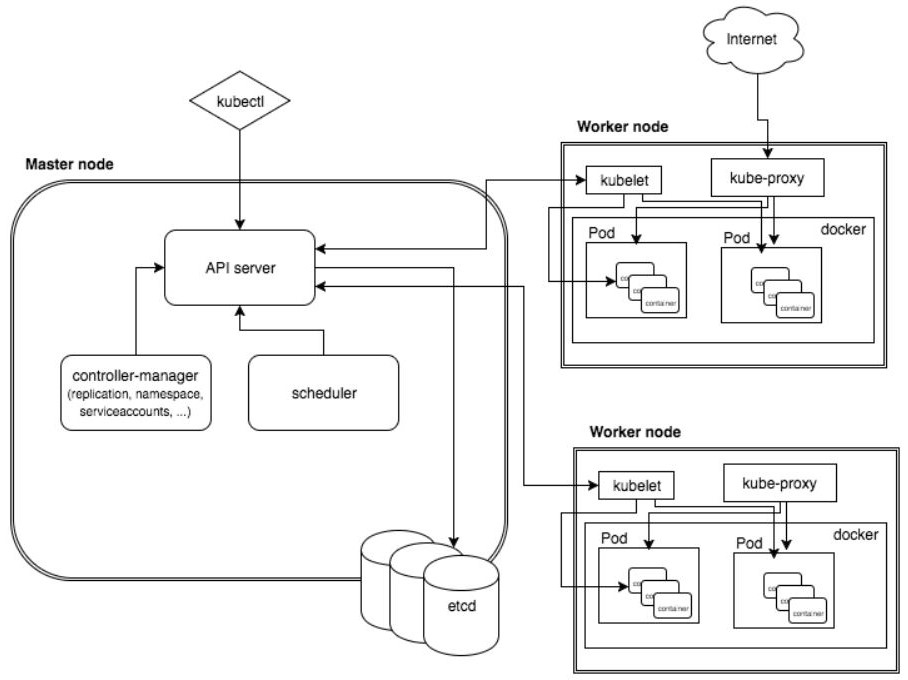
\includegraphics[width=0.7\textwidth]{resources/k8s_architecture}
	\caption[Architecture Diagram of K8s]{This diagram illustrates the main parts: The \textit{master node} representing the central unit for the orchestration of the Kubernetes cluster. The \textit{worker nodes} running the user-specified workloads represented as \textit{pods} on the Kubernetes cluster. The cluster can be controller and orchestrated by the user using the \textit{kubectl}-CLI. \cite{K8sArch}}
	\label{k8s_architecture}
\end{figure}
K8s consist of three main components \textit{kubectl}, \textit{master node}, and the \textit{worker nodes}. Kubectl represents the client interface to communicate with the master node, by sending requests against the API server. The master node represents the administrative entrypoint and is responsible for managing the whole K8s cluster \cite{K8sArch}. It consists of the \textit{API server}, \textit{etcd storage}, \textit{scheduler}, and \textit{controller manager}:

\begin{itemize}
	\item \textit{API server} represents the entry points for all incoming REST commands. It processes and executes them according to their business logic.
	\item \textit{etcd storage} is a simple key-value store, where information about the \textit{pods} and the cluster is saved.
	\item \textit{scheduler} is responsible for container distribution among the worker nodes by using information about the worker nodes. 
	\item \textit{controller-manager} consists of several controllers such as the replication controller, which is responsible for monitoring pods and recreating crashed pods.
\end{itemize}
Beside the master node, a K8s cluster consists of one or more worker nodes, which are controller by the controllers of the master node. Each worker node consists of \textit{kubelet}, \textit{kubeproxy}, and \textit{pods}:

\begin{itemize}
	\item \textit{kubelet} communicates with the API server, ensuring the requested containers are up and running.
	\item \textit{kube-proxy} acts as a proxy and load balancer on the worker node. It is responsible for the communication with the outside world.
	\item \textit{pods} is the smallest unit in K8s. They encapsulate one or many other containers in the same shared context, which means that containers within the same pods share the same IP, storage, and memory.
\end{itemize}


\section{Method}
Our contributions, novel aspects, great detail


\section{Datasets}
In our approach we propose a supervised machine learning algorithm to estimate the page rank using deep graph networks. For this purpose we require labelled data to develop, train and validate our model. 

In general the process of gathering, augmenting and labelling of data can take an immense amount of time and slow down the development of machine learning model. Therefore we decided to iteratively develop and align our dataset to the current need of research and progress of development. For each upcoming iteration we specified the requirements for the data set. Following from this each iteration resulted in an own data set version.

The following sections will profoundly specify each dataset version as required during the development of our approach.

\subsection{Dataset Version 1}
\label{DatasetVersion1}
The dataset version 1 consists of 100000 samples in total. The ground truth for this dataset version is \textit{OpenPage Rank}, which is described in \ref{OpenPageRank}.

Every sample $k$ is a tuple consisting of three values and corresponds to one Domain $D$ from the ground truth:

\begin{center}
 $ k \in (I_D, R_D, U_D)$
\begin{itemize}
	\item[$I_D$]: The screenshot of the domain $D$ in image format PNG and in the resolution 1920x1080.
	\item[$R_D$] $\in [1, 100000]$ : The global rank of the domain $D$, according to Open PageRank (\ref{OpenPageRank}). 
	\item[$U_D$]: The URL of the domain $D$ mapped by the Open PageRank list. Example: \textit{github.com}
\end{itemize}
\end{center}

\subsection{Dataset Version 2}
\label{DatasetVersion2}
The dataset version 2 consists of 100000 samples in total and the ground truth is \textit{Open PageRank} as described in dataset version 1.

Every sample $k$ is mapped to a domain $D$ from the ground truth and represents a tuple consisting of four values:

\begin{center}
$k \in (U_D,R_D,H_D,G_D)$
\begin{itemize}
	 \item[$U_D$]: The URL of the domain $D$ mapped by the Open PageRank list.
	\item[$R_D$] $\in [1, 100000]$ : The global rank of the domain $D$ according to Open PageRank (\ref{OpenPageRank}). 
    \item[$H_D$] $\in \{true, false\}$: Indicator for whether the website uses the protocol HTTPS.
    \item[$G_D$] $= (V_D, A_D)$: The directed graph of the domain $D$ characterized by a set of vertices $V_D$ and arrows $A_D$.
\end{itemize}
\end{center}

\subsubsection{The Directed Graph}
The directed graph provides a topological view on the given website by representing all associated webpages within the same domain as vertices and connections as arrows as in figure \ref{fig:PartialDirectedGraph_timodenk.com} exemplary illustrated. During the crawling process as described in \ref{Datacrawler} vertices and arrows of the graph are created and enriched with local information about the visited webpages.

The directed graph $G_D$ is characterized by a set of vertices $V_D$ and arrows $A_D$. Each vertices $v \in V_D$ represents a webpage $p$ of the given domain $D$ and is characterized by the following tuple:

\begin{center}
	$v \in (U_p, I_p, M_p,T_p, L_p, S_p)$
\begin{itemize}
	\item[$ U_p$] : The exact URL of the webpage $p$. Example: \textit{https://github.com/help}
	\item[$I_p$] : The screenshot of webpage $p$ in image format PNG and in the resolution 1920x1080.
	\item[$M_p$] The screenshot of webpage $p$ in image format PNG and in mobile resolution TODO ZxY.
	\item[$T_p$] : The title of webpage $p$ as can be seen in the tabs bar of a common browser.
	\item[$L_p$] : The time it takes to download all data of webpage $p$ from the web server in milliseconds.
	\item[$S_p$] : Number of kilobytes downloaded in total for webpage $p$.
\end{itemize}
\end{center}

Each arrow represents a possible navigation from webpage $p$ to $q$ in the graph $G_D$. It can be understood as a hyperlink or button found on webpage $p$ (source), which leads to webpage $q$ (target) in the same domain $G_D$. 

\begin{center}
	$a \in (U_p, U_q, L_{p,q})$
	\begin{itemize}
		\item[$U_p$] : The source URL of the webpage $p$
		\item[$U_q$] : The target URL of the webpage $q$ the arrow directs to.
		\item[$L_{p,q}$] : If existent, the text that links from source to target webpage. 
	\end{itemize}
\end{center}

\begin{figure}
\centering
\usetikzlibrary{shapes.multipart}
  \tikzset{
	vertices/.style = {   
		text width=12.0em, align=center,                                           
		draw,
		rectangle split,
		rectangle split parts=6
	}
}
\scalebox{.85}{
\begin{tikzpicture}
\node[vertices]  (timodenk) at (5,4) {
	\nodepart{one} timodenk.com 
	\nodepart{two} 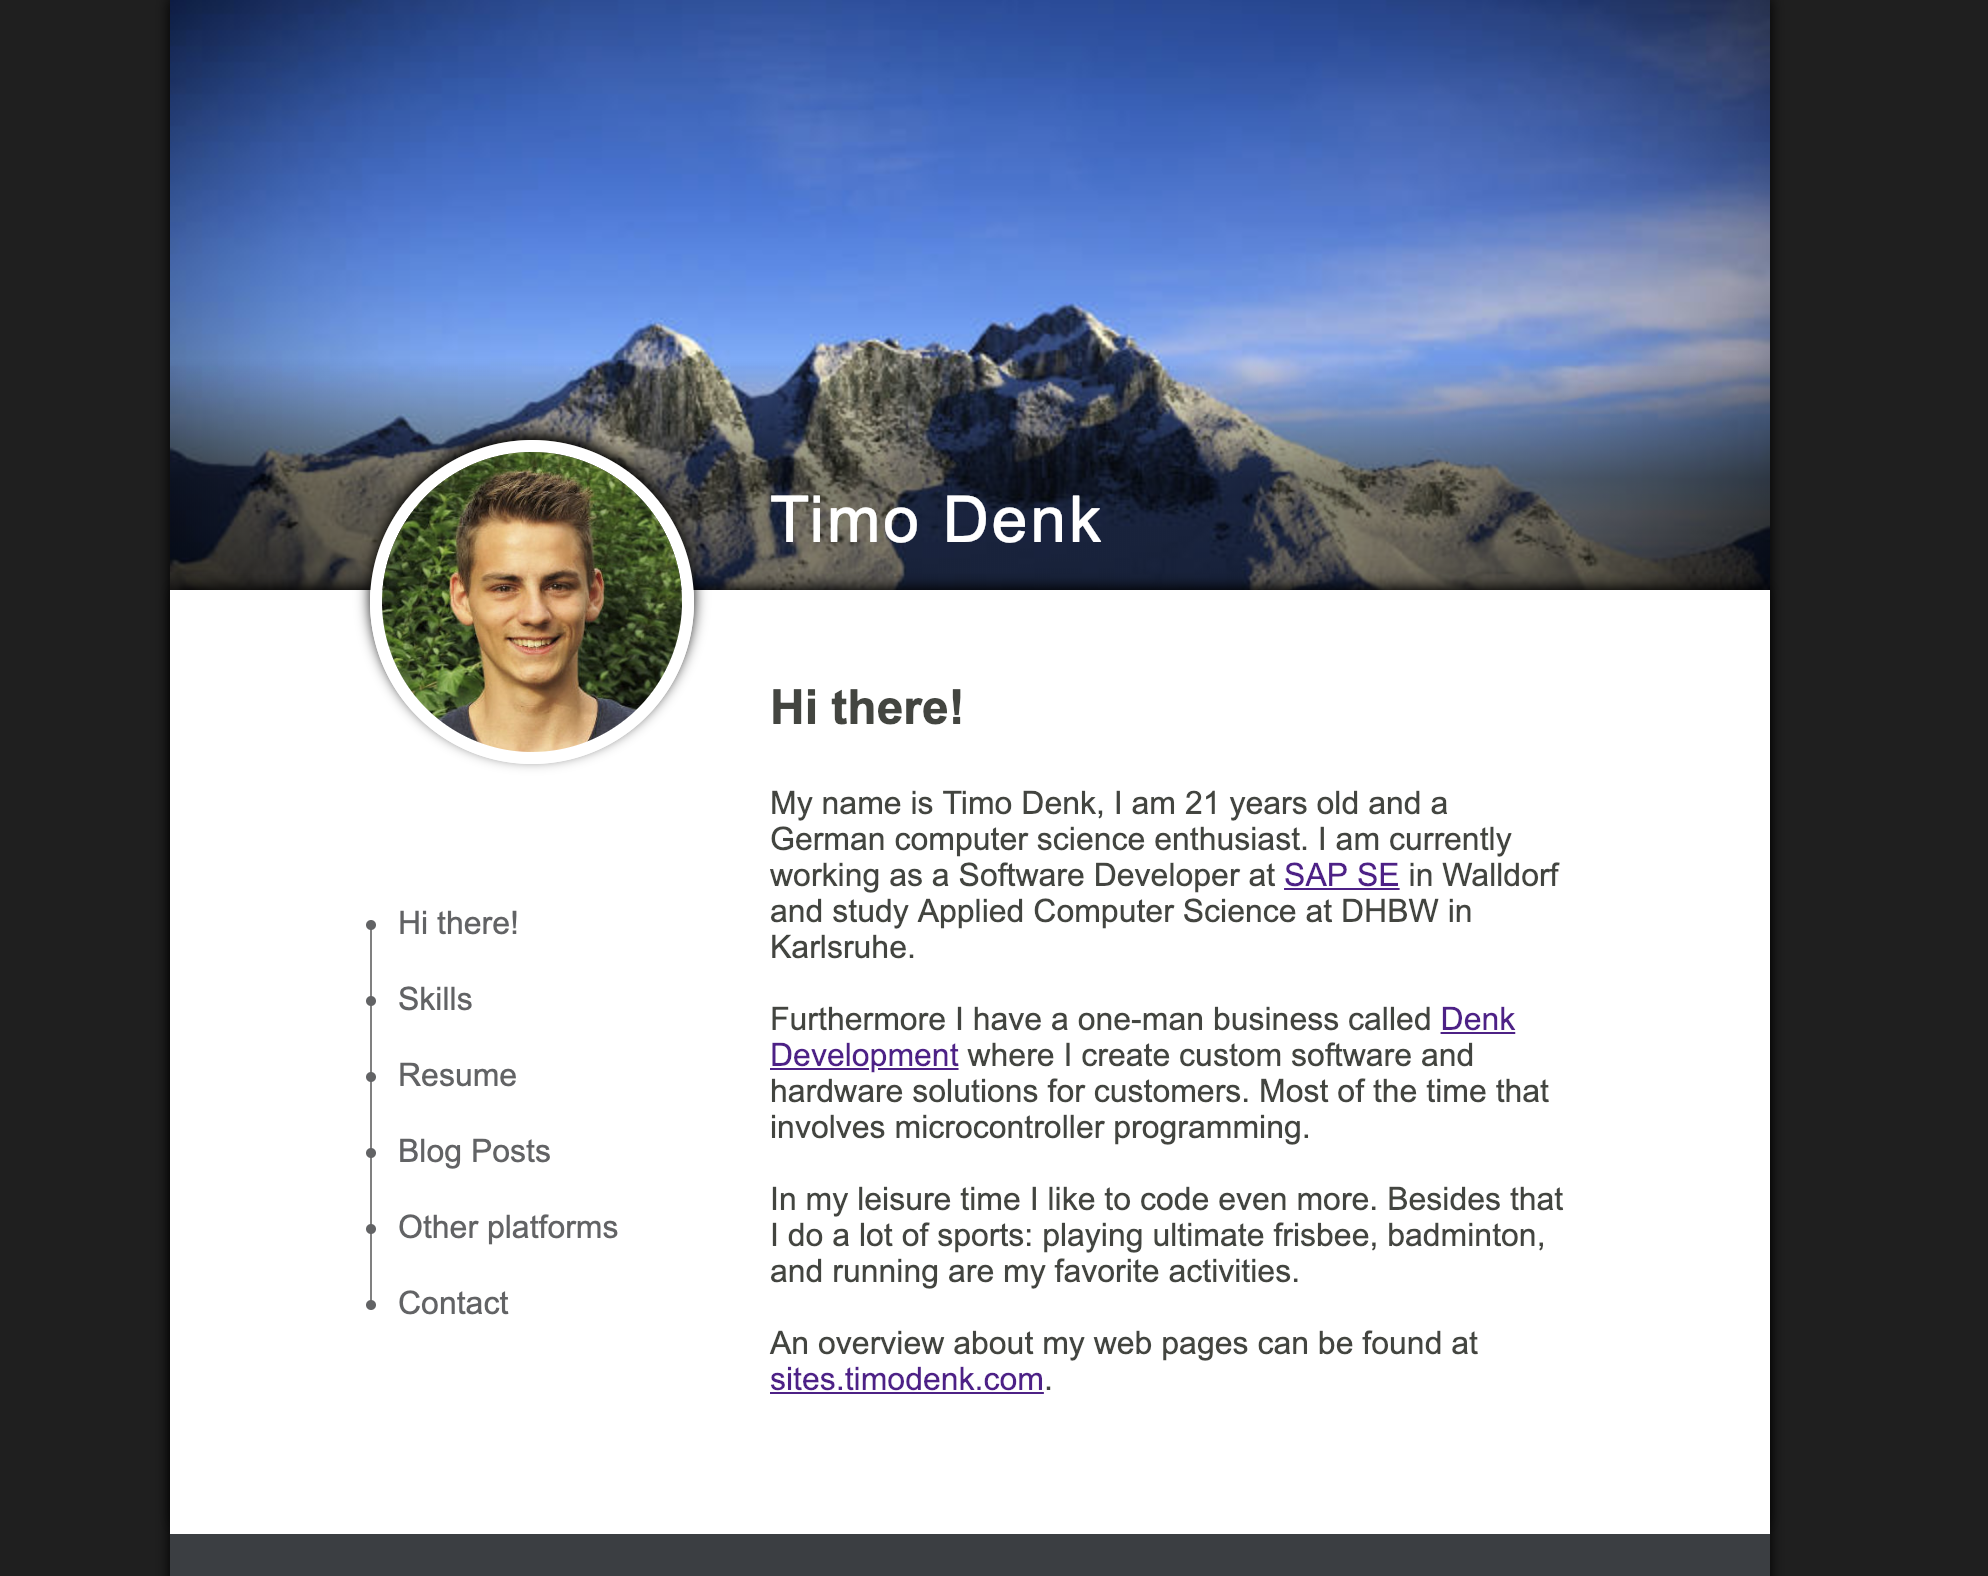
\includegraphics[width=.5\textwidth]{resources/timodenk}
	\nodepart{three} 
\includegraphics[width=.25\textwidth]{resources/timodenk_mobile}
	\nodepart{four} Timo Denk
	\nodepart{five} 636 ms
	\nodepart{six} 434 kb
};

\node[vertices]  (sites) at (10,2) {
\nodepart{one} sites.timodenk.com
\nodepart{two} 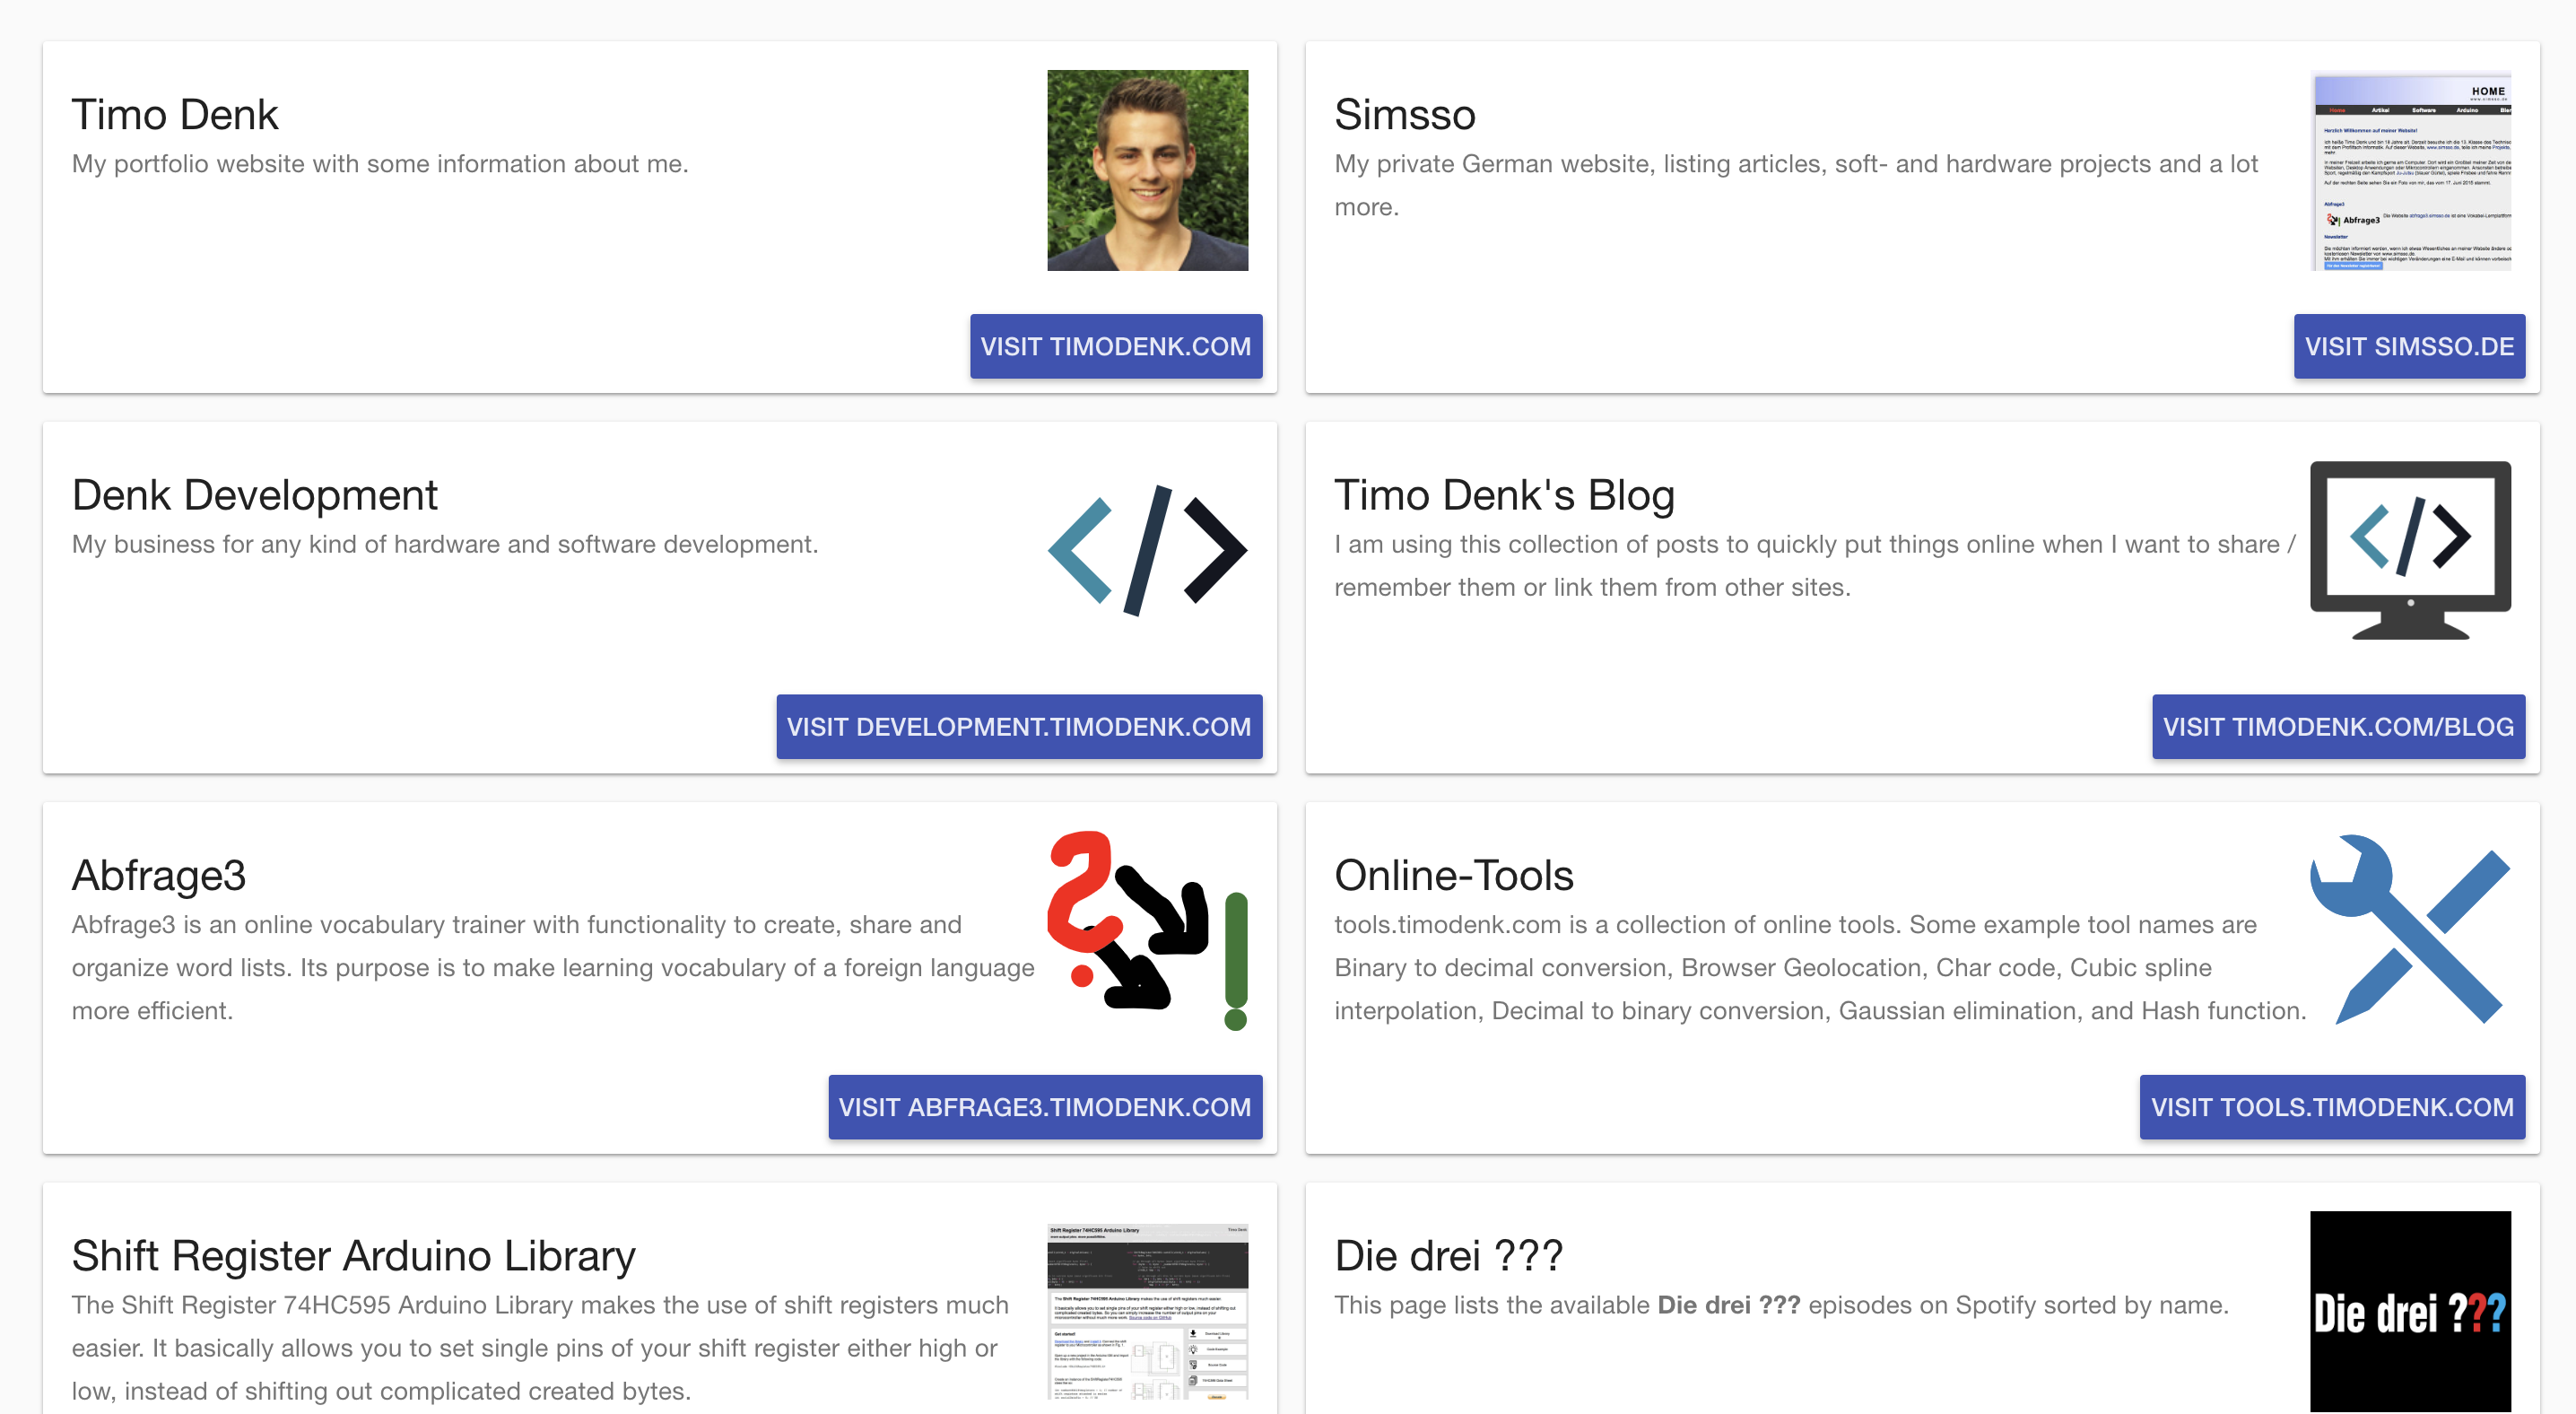
\includegraphics[width=.5\textwidth]{resources/sites_timodenk}
\nodepart{three} 
\includegraphics[width=.25\textwidth]{resources/sites_timodenk_mobile}	\nodepart{four} Timo Denk Sites Overview
\nodepart{five} 767 ms
\nodepart{six} 737 kb
};

\node[vertices]  (imprint) at (0,2) {
\nodepart{one} timodenk.com/imprint
\nodepart{two} 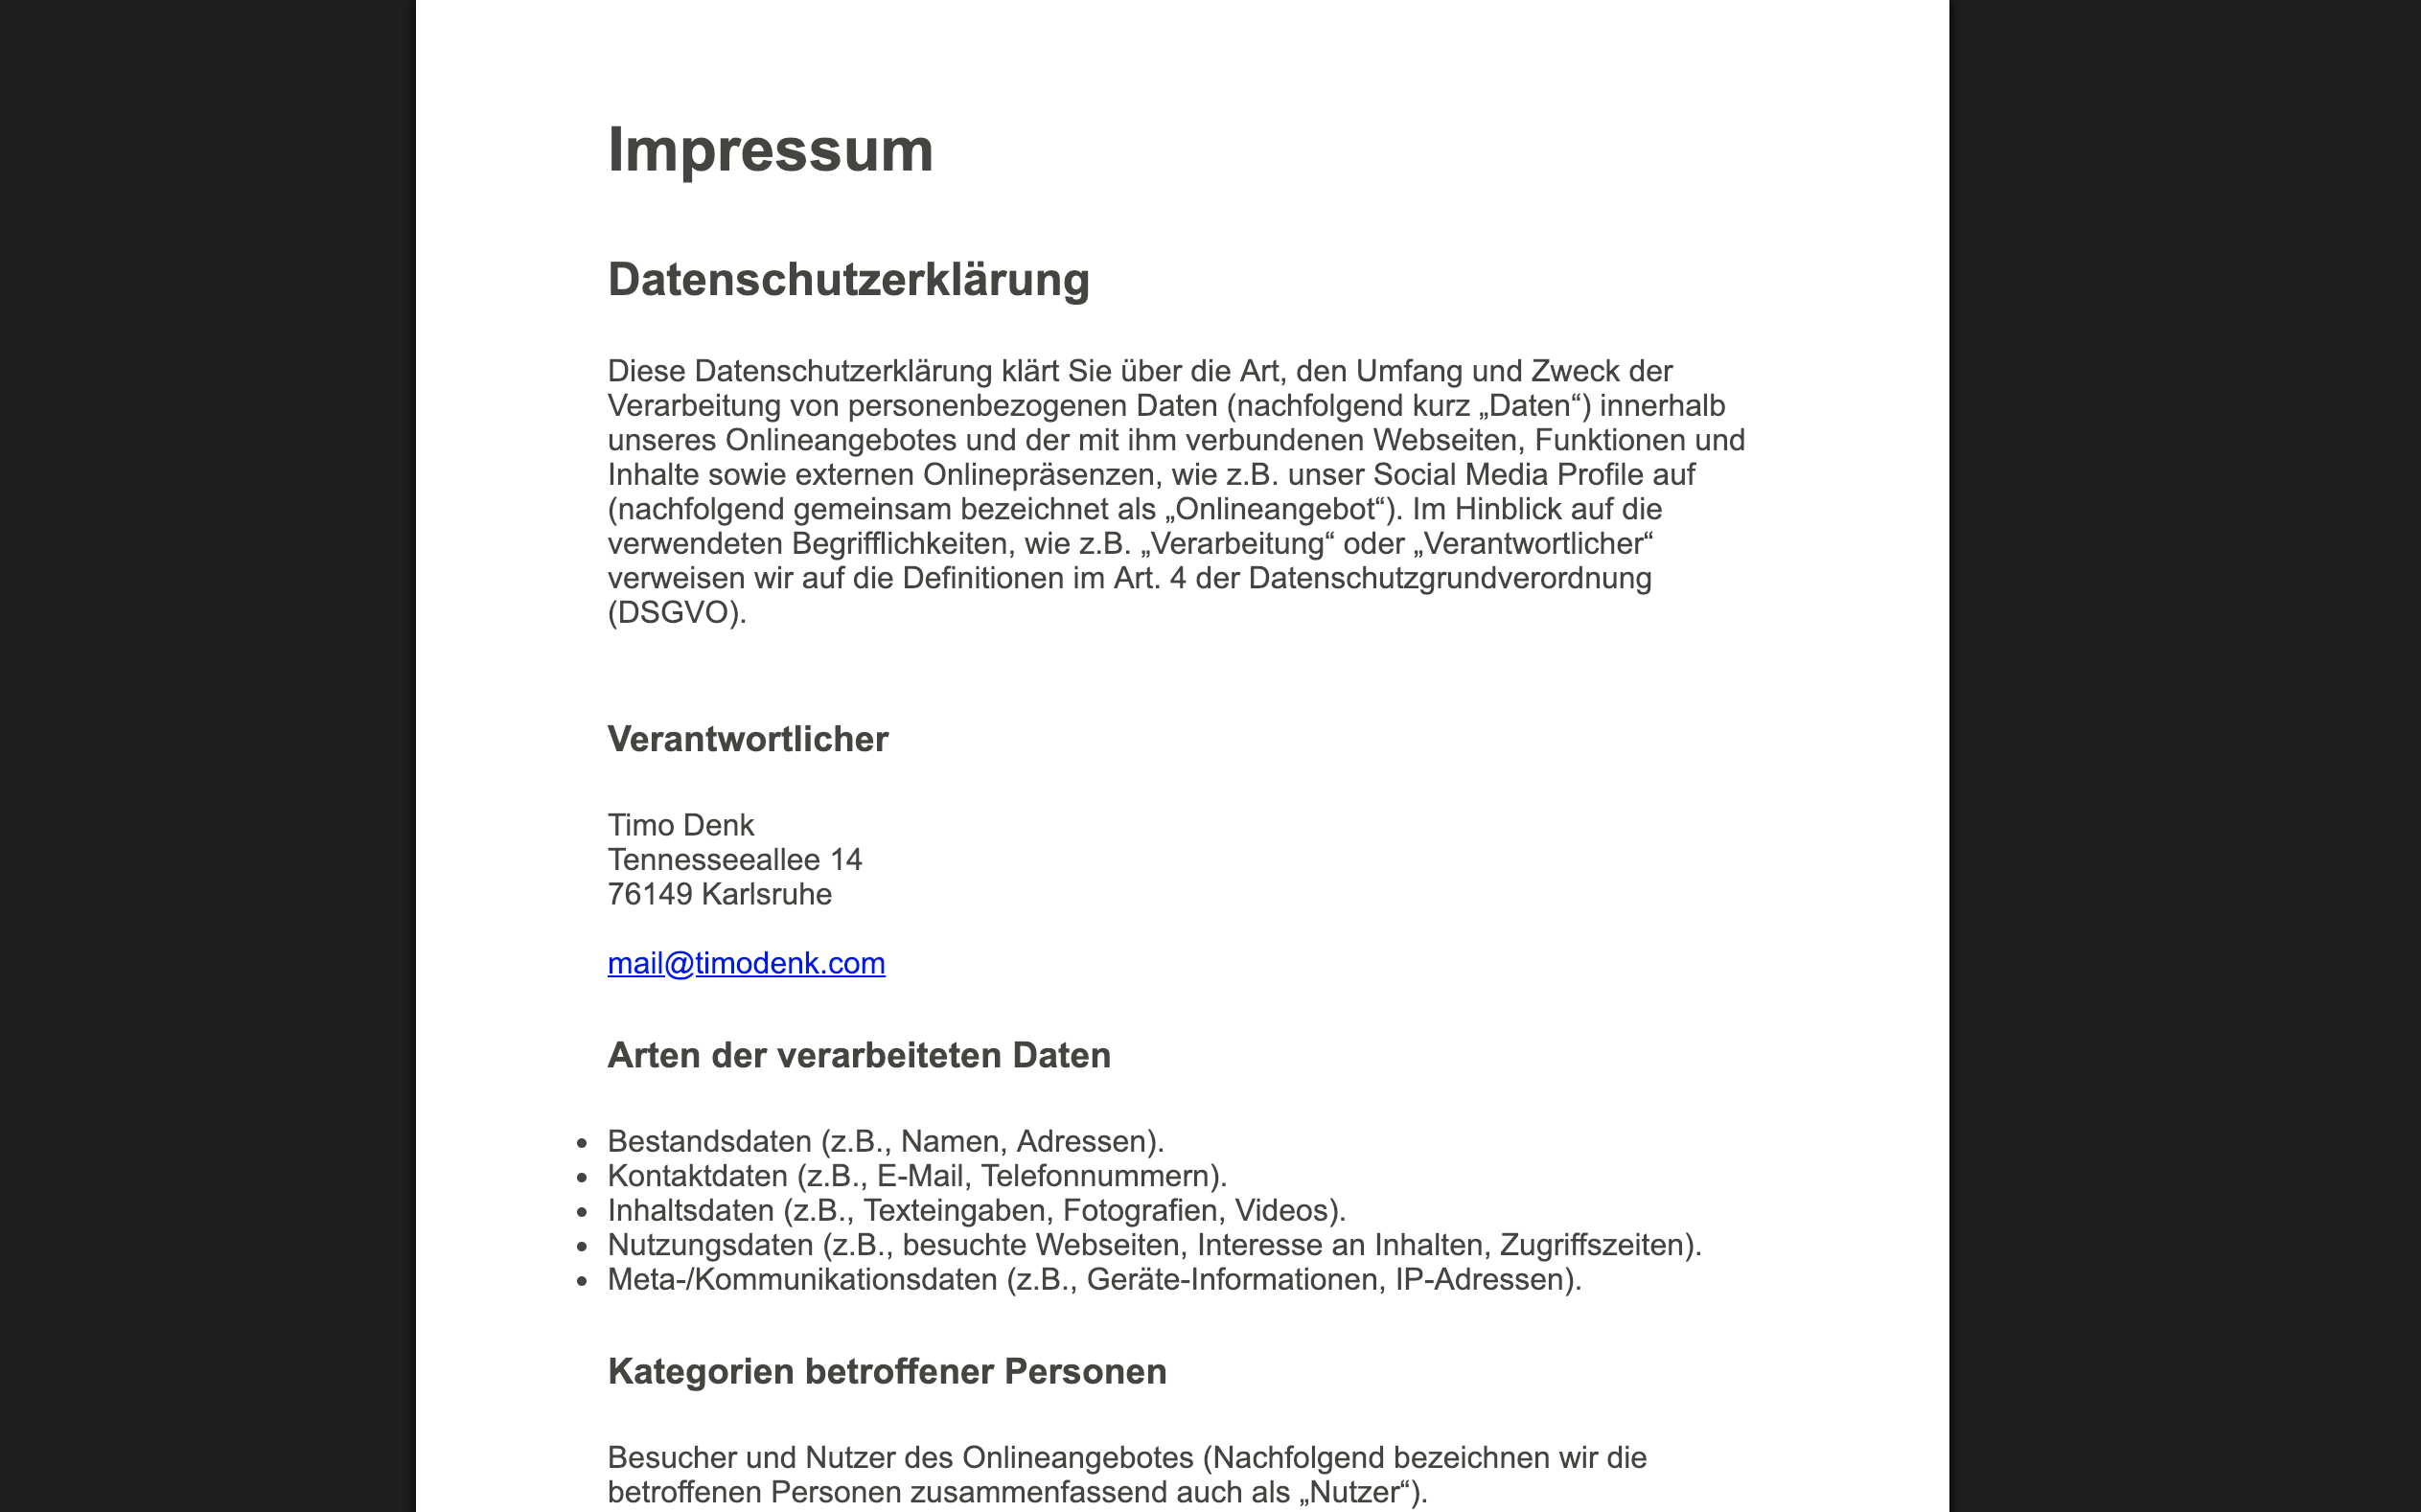
\includegraphics[width=.5\textwidth]{resources/imprint_timodenk}
\nodepart{three} 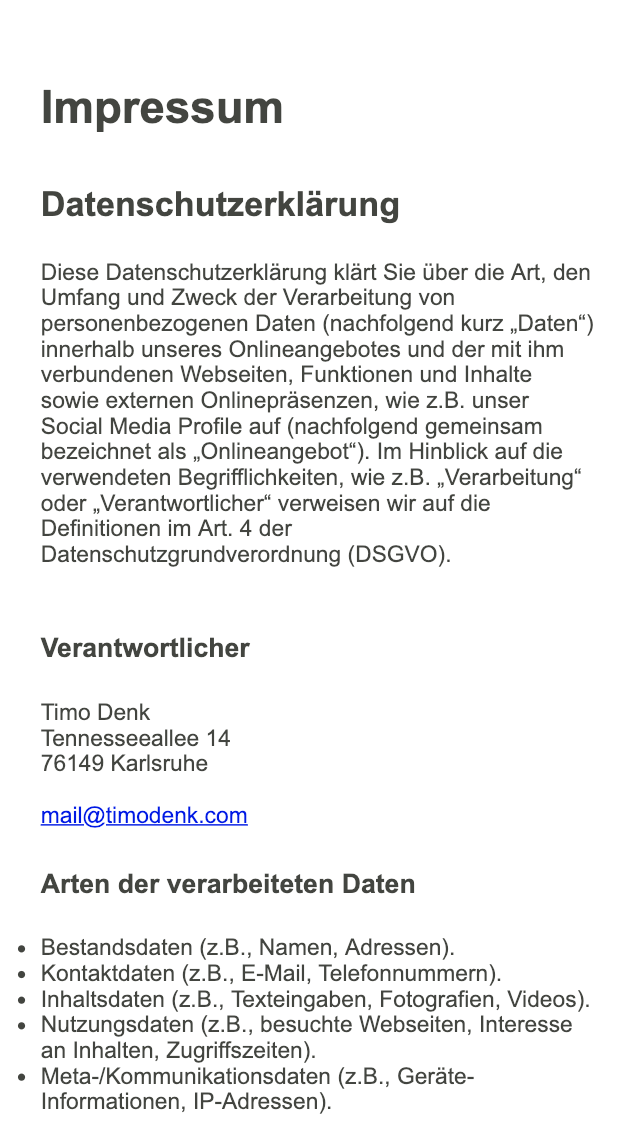
\includegraphics[width=.25\textwidth]{resources/imprint_timodenk_mobile}
\nodepart{four} Imprint - www.timodenk.com
\nodepart{five} 304 ms
\nodepart{six} 52 kb
};

\node (timodenkToImprint) at (0.5,6) {timodenk.com/imprint};
\node (timodenkToSites) at (9.5,6) {sites.timodenk.com};
\node (SitesToTimodenk) at (5.5,0.25) {timodenk.com};
\draw[-latex] (timodenk.one east) to [bend left=30] (sites.one north);
\draw[-latex] (sites.six west) to [bend left=30] (timodenk.six south);
\draw[-latex] (timodenk.one west) to [bend right=30](imprint.one north);
\end{tikzpicture}
}
\caption{Illustrates partial directed graph of domain \textit{timodenk.com} with three webpages, corresponding arrows and vertices}
\label{fig:PartialDirectedGraph_timodenk.com}
\end{figure}


\section{Implementation Details}
Technical aspects of our methods, things we have tried that might have failed, code snippets
Technical description of the dataset creation process

\section{Results}
Presentation of our results, no opinion

\section{Discussion}
Discussion of the results, assumptions about why things are the way they are

\section{Conclusion}
Summary, outlook, future work

\printbibliography
\addcontentsline{toc}{section}{References}
\label{sec:references}

\end{document}
